\documentclass[11pt]{article}
\usepackage[utf8]{inputenc}
\usepackage{geometry, wrapfig, float, multicol, mathtools, array, csquotes, lscape, setspace}
\usepackage[sorting=nty]{biblatex}
\addbibresource{bibliography.bib}
\usepackage[font=small,labelfont=bf]{caption}
\usepackage{multicol}
\usepackage[demo]{graphicx}

\geometry{
    top=3.5cm,
    bottom=3.0cm,
    outer=2.5cm,
    inner=2.5cm
}
\setlength{\columnsep}{0.8cm}
\setlength{\parindent}{0pt}
\setlength{\skip\footins}{20pt}

\newenvironment{Figure}
  {\par\medskip\noindent\minipage{\linewidth}}
  {\endminipage\par\medskip}

\title{Comparative Analysis of Convolutional Neural Network and ScatNet for Brain Tumor Classification in Medical Images: A Study on Performance and Explainability}
\author{Virginia Filippi - VR495315, Alberto Righetti - VR495554, Chiara Solito - VR487795}
\date{}

\begin{document}

\maketitle

\begin{abstract}
This project aims to compare the performances of a 2D Convolutional Neural Network (CNN) and a Scattering Network for classifying brain tumors in MRI images. Filters were extracted for each network, and their performance was analyzed as the dataset size varied. The study also includes an explainability analysis using various eXplainable Artificial Intelligence (XAI) methods: Integrated Gradients algorithm from scratch, Captum library's version, and LIME, to highlight relevant areas in image classification, visualizing attribution maps and performing different statistical analyses on them.
\end{abstract}

\begin{multicols*}{2}

\section{Introduction}
The advent of deep learning has revolutionized many fields, including medical imaging, where deep techniques have shown remarkable performance in tasks like image classification, segmentation, and detection. However, despite their success, these models often act as black boxes, making their predictions difficult to interpret. This lack of transparency, known as the problem of explainability, is particularly concerning in the medical field, where understanding the reasoning behind a model’s prediction is crucial for trust and actionable insights.

In this context, our project aims to bridge the gap between performance and interpretability in medical imaging models. We first provide a comparative study of Convolutional Neural Network (CNN) and ScatNet, two popular deep learning techniques in medical imaging. We then introduce explainable algorithms, specifically Integrated Gradients and Local Interpretable Model-Agnostic Explanations (LIME), to shed light on the decision-making process of these models. By doing so, we hope to make these powerful tools more accessible and trustworthy for healthcare professionals, ultimately leading to better patient outcomes.

In the following sections, we will delve deeper into the technical aspects of these models and explainable algorithms, followed by a detailed discussion of our experimental setup, results, and their implications in the medical field.

\section{Dataset Selection}
The dataset chosen for the project is a collection of magnetic resonance images divided into two classes: without tumor (class 0) and with tumor (class 1). The original dataset was comprehensive of different classes of tumors, but we decided to make the task a binary classification. \footnote{Link: https://www.kaggle.com/datasets/masoudnickparvar/brain-tumor-mri-dataset}. The dataset is composed of 3200 MRI images, 2600 for training, and 600 for testing, with a balanced proportion of the two classes for both training and testing datasets.

\subsection{Data pre-processing}
For each image, we have done a preprocessing step based on the following transforms: the conversion into PIL Image, the resizing of all the images to a uniform size of 128x128 pixels, the conversion to \texttt{Pytorch} tensor, and finally the normalization with mean and standard deviations for each channel, computed on all the dataset images. 

To improve the generalization capacity of the networks, data augmentation was applied by tripling the number of images of the train dataset, for a total number of 7800 images divided for training and validation.
The following transformations were applied for data augmentation: random rotations (randomly with degrees from 0 to 90) and horizontal and vertical flips (randomly with probability 0.1).


\subsection{K-Fold Cross Validation}
The splitting of the training data into training and validation was implemented using the K-Fold cross-validation technique for the training phase. 
K-fold cross-validation is a machine learning technique to assess the performance of a model. It involves dividing the dataset into k subsets, iteratively training the model on k-1 subsets and validating on the remaining subset. This technique offers advantages such as maximizing data usage, providing reliable performance estimates, assessing model robustness and evaluating generalization ability of a model averaging the performance metrics obtained from each iteration.

In particular, the \texttt{Stratified K-Fold} function of the \texttt{scikit-learn} library was used to divide the dataset into 10 different folds, which is considered one of the standard and optimal numbers for k-fold cross-validation.

\section{Methodology}
\subsection{Convolutional Neural Network}

A Convolutional Neural Network (CNN) is an artificial neural network specifically designed for analyzing visual data. It's structured to automatically and adaptively learn spatial hierarchies of features from input images.

By leveraging convolutional operations and hierarchical feature learning, CNNs have become a cornerstone in various computer vision tasks such as image classification, object detection, facial recognition, and more.

Our implementation follows a standard version of the CNN, let's delve deeper into our architecture and our training.

\subsubsection{The architecture}
The convolutional neural network (CNN) is structured with four convolutional layers, initializing the initial parameters of the layers with values using a Xavier normal distribution. The convolutional layers are strategically interleaved with max-pooling operations and rectified linear unit (ReLU) activations. Batch normalization layers have been added for every 2 convolution layers. These convolutional layers act as feature extractors, capturing increasingly sophisticated patterns from the input data.

Following this convolutional stack, the architecture transitions into a linear classifier with a transitional flattening layer. Comprising three fully connected layers, this segment refines the extracted features for effective classification. To mitigate overfitting, two dropout layers were introduced, randomly deactivating a fraction of units during training (with probabilities $p=0.3$ and $p=0.1$).

\begin{Figure}
    \centering
    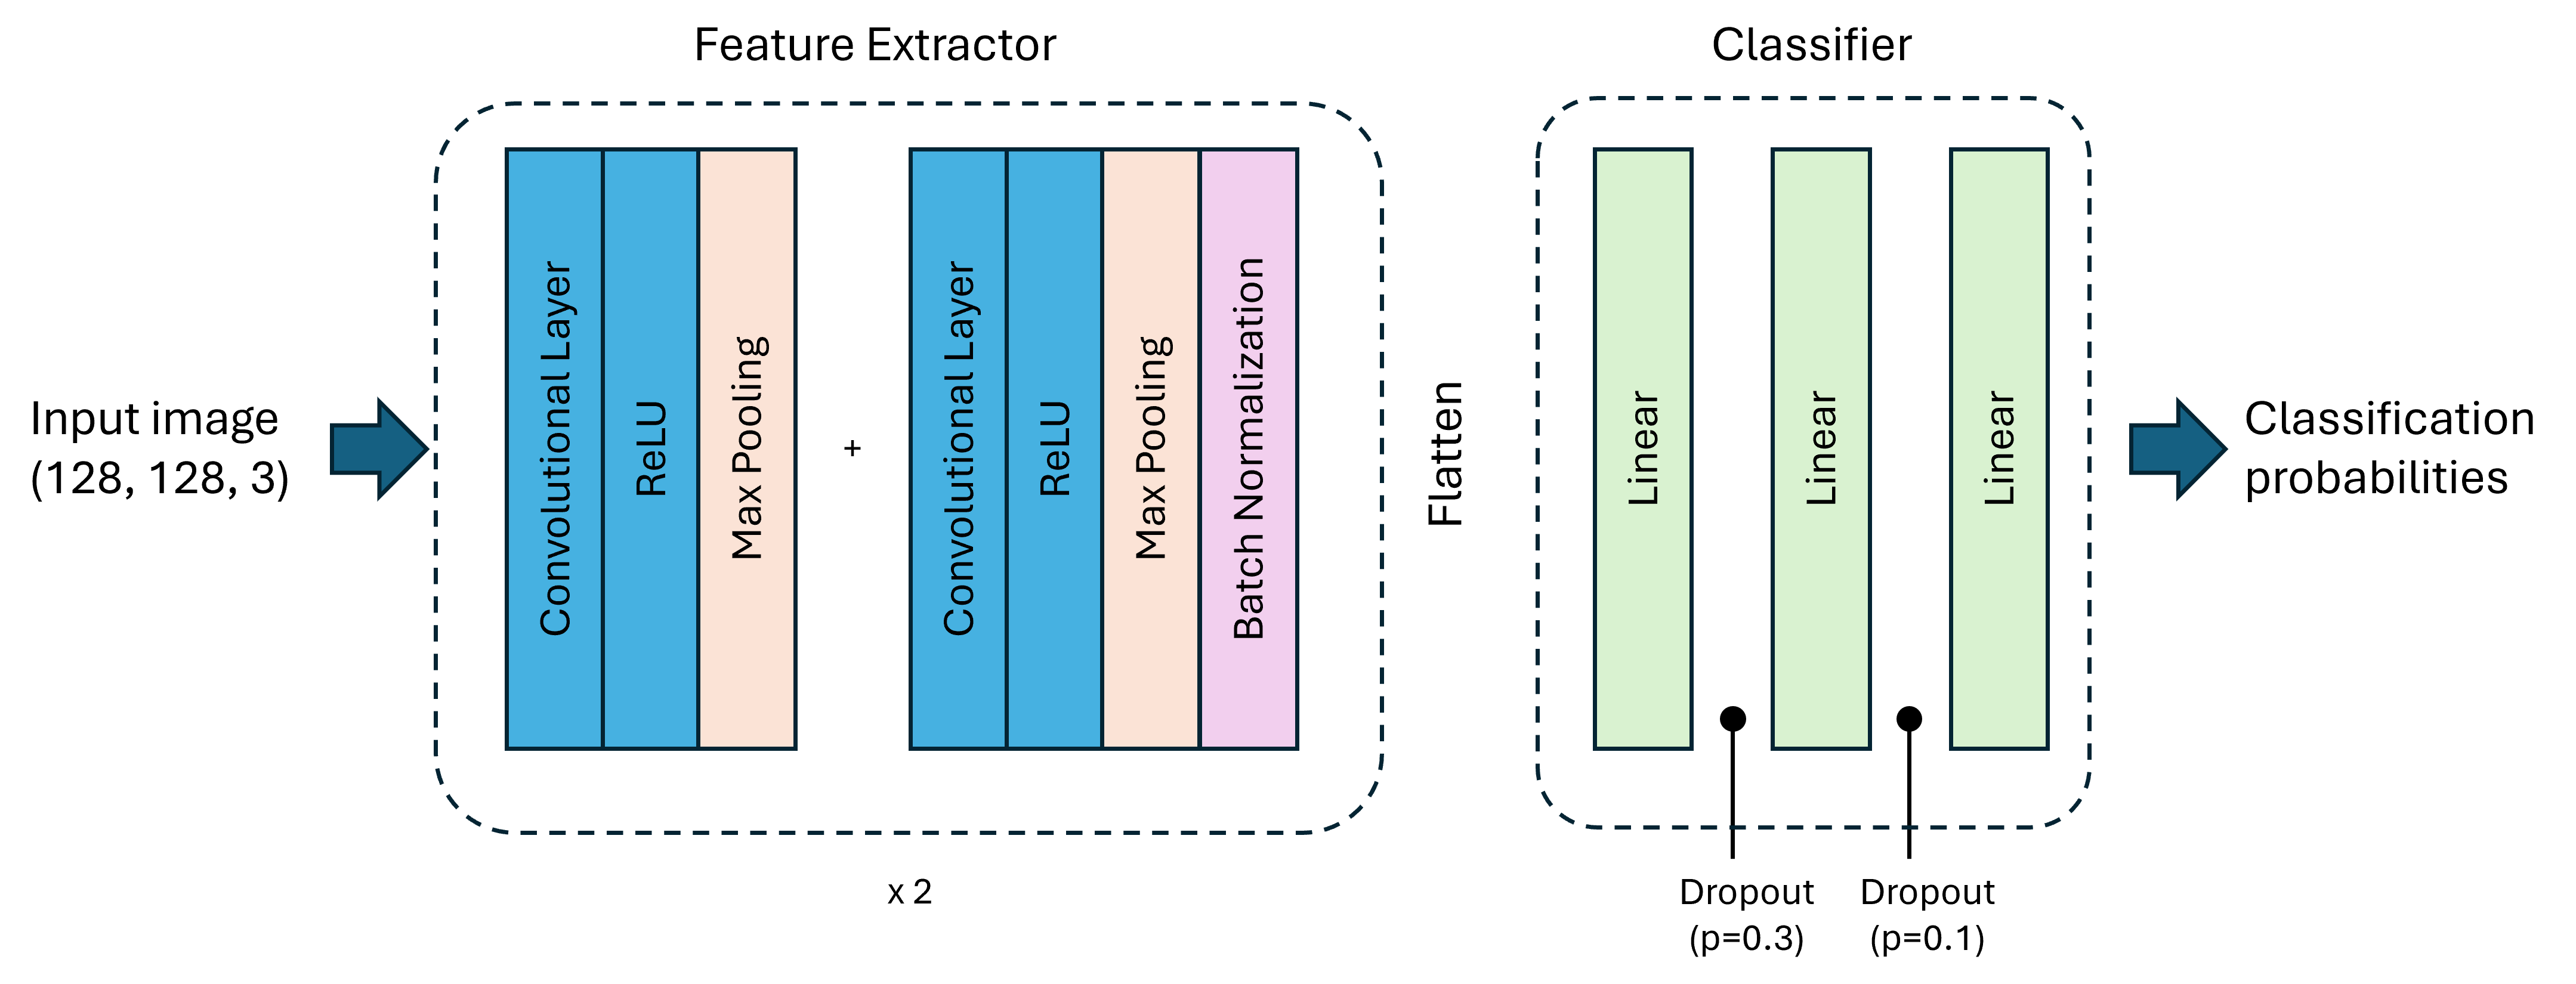
\includegraphics[width=\linewidth]{images/cnn_architecture.png}
    \captionof{figure}{CNN architecture}
    \label{fig:cnn-architecture}
\end{Figure}


\subsection{ScatNet}
The Scattering Network (ScatNet) employs a distinct architecture tailored for robust feature extraction in image classification tasks. It is a powerful tool in signal processing and deep learning, particularly for analyzing and extracting features from images and other types of signals.

The key concept of Scattering Transform is to extract the same information for the same class, which has many variations between each image belonging to it. The Scattering Transform is invariant in transformation so it can extract similar main features from images of the same class, where the class is translated or deformated. The process is divided into stages, each one consisting of a convolution, a non-linear operation (usually modulus), and the averaging. It is also important to specify the number of scales that will be used and in the case of images even the number of angles in which the wavelet will be rotated.

\begin{Figure}
    \centering
    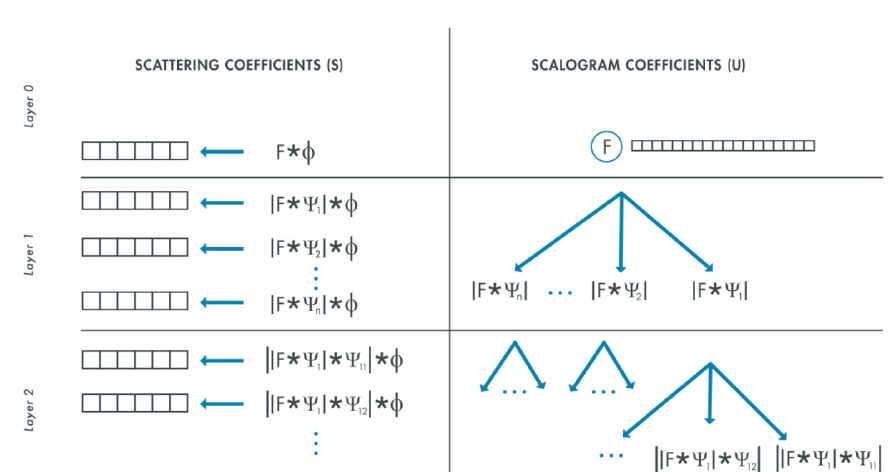
\includegraphics[width=\linewidth,height=4cm]
    {images/scatnet_flow_better_image.png}
    \captionof{figure}{Wavelet scattering transform flow; $\psi_j$ are the wavelets, $\phi$ is the scaling function and $f$ is the input data.}
    \label{fig:scatnet-flow}
\end{Figure}

The above picture shows the process for feature extraction performed by ScatNet. When images are used as input data for each $\psi_j$ there are a number of rotations of wavelet associated. The nodes of the tree represent the Scalogram Coefficients, which are convolved with scaling function $\phi$, to generate the Scattering coefficients. The whole set of Scattering Coefficients are the low-variance features that are extracted from the data.


\subsubsection{The architecture}
The core component is a scattering layer, implemented using the Scattering2D function from the \texttt{Kymatio} library. This layer captures essential information about the input images, facilitating translation-invariant feature learning.

Following the scattering layer, the architecture transitions into a linear layer that refines the extracted features. This linear layer bridges the subsequent linear classifier, which comprises three fully connected layers. The linear classifier is equal to that in the CNN architecture (as project instructions), fine-tuning the abstracted features for accurate classification.

\begin{Figure}
    \centering
    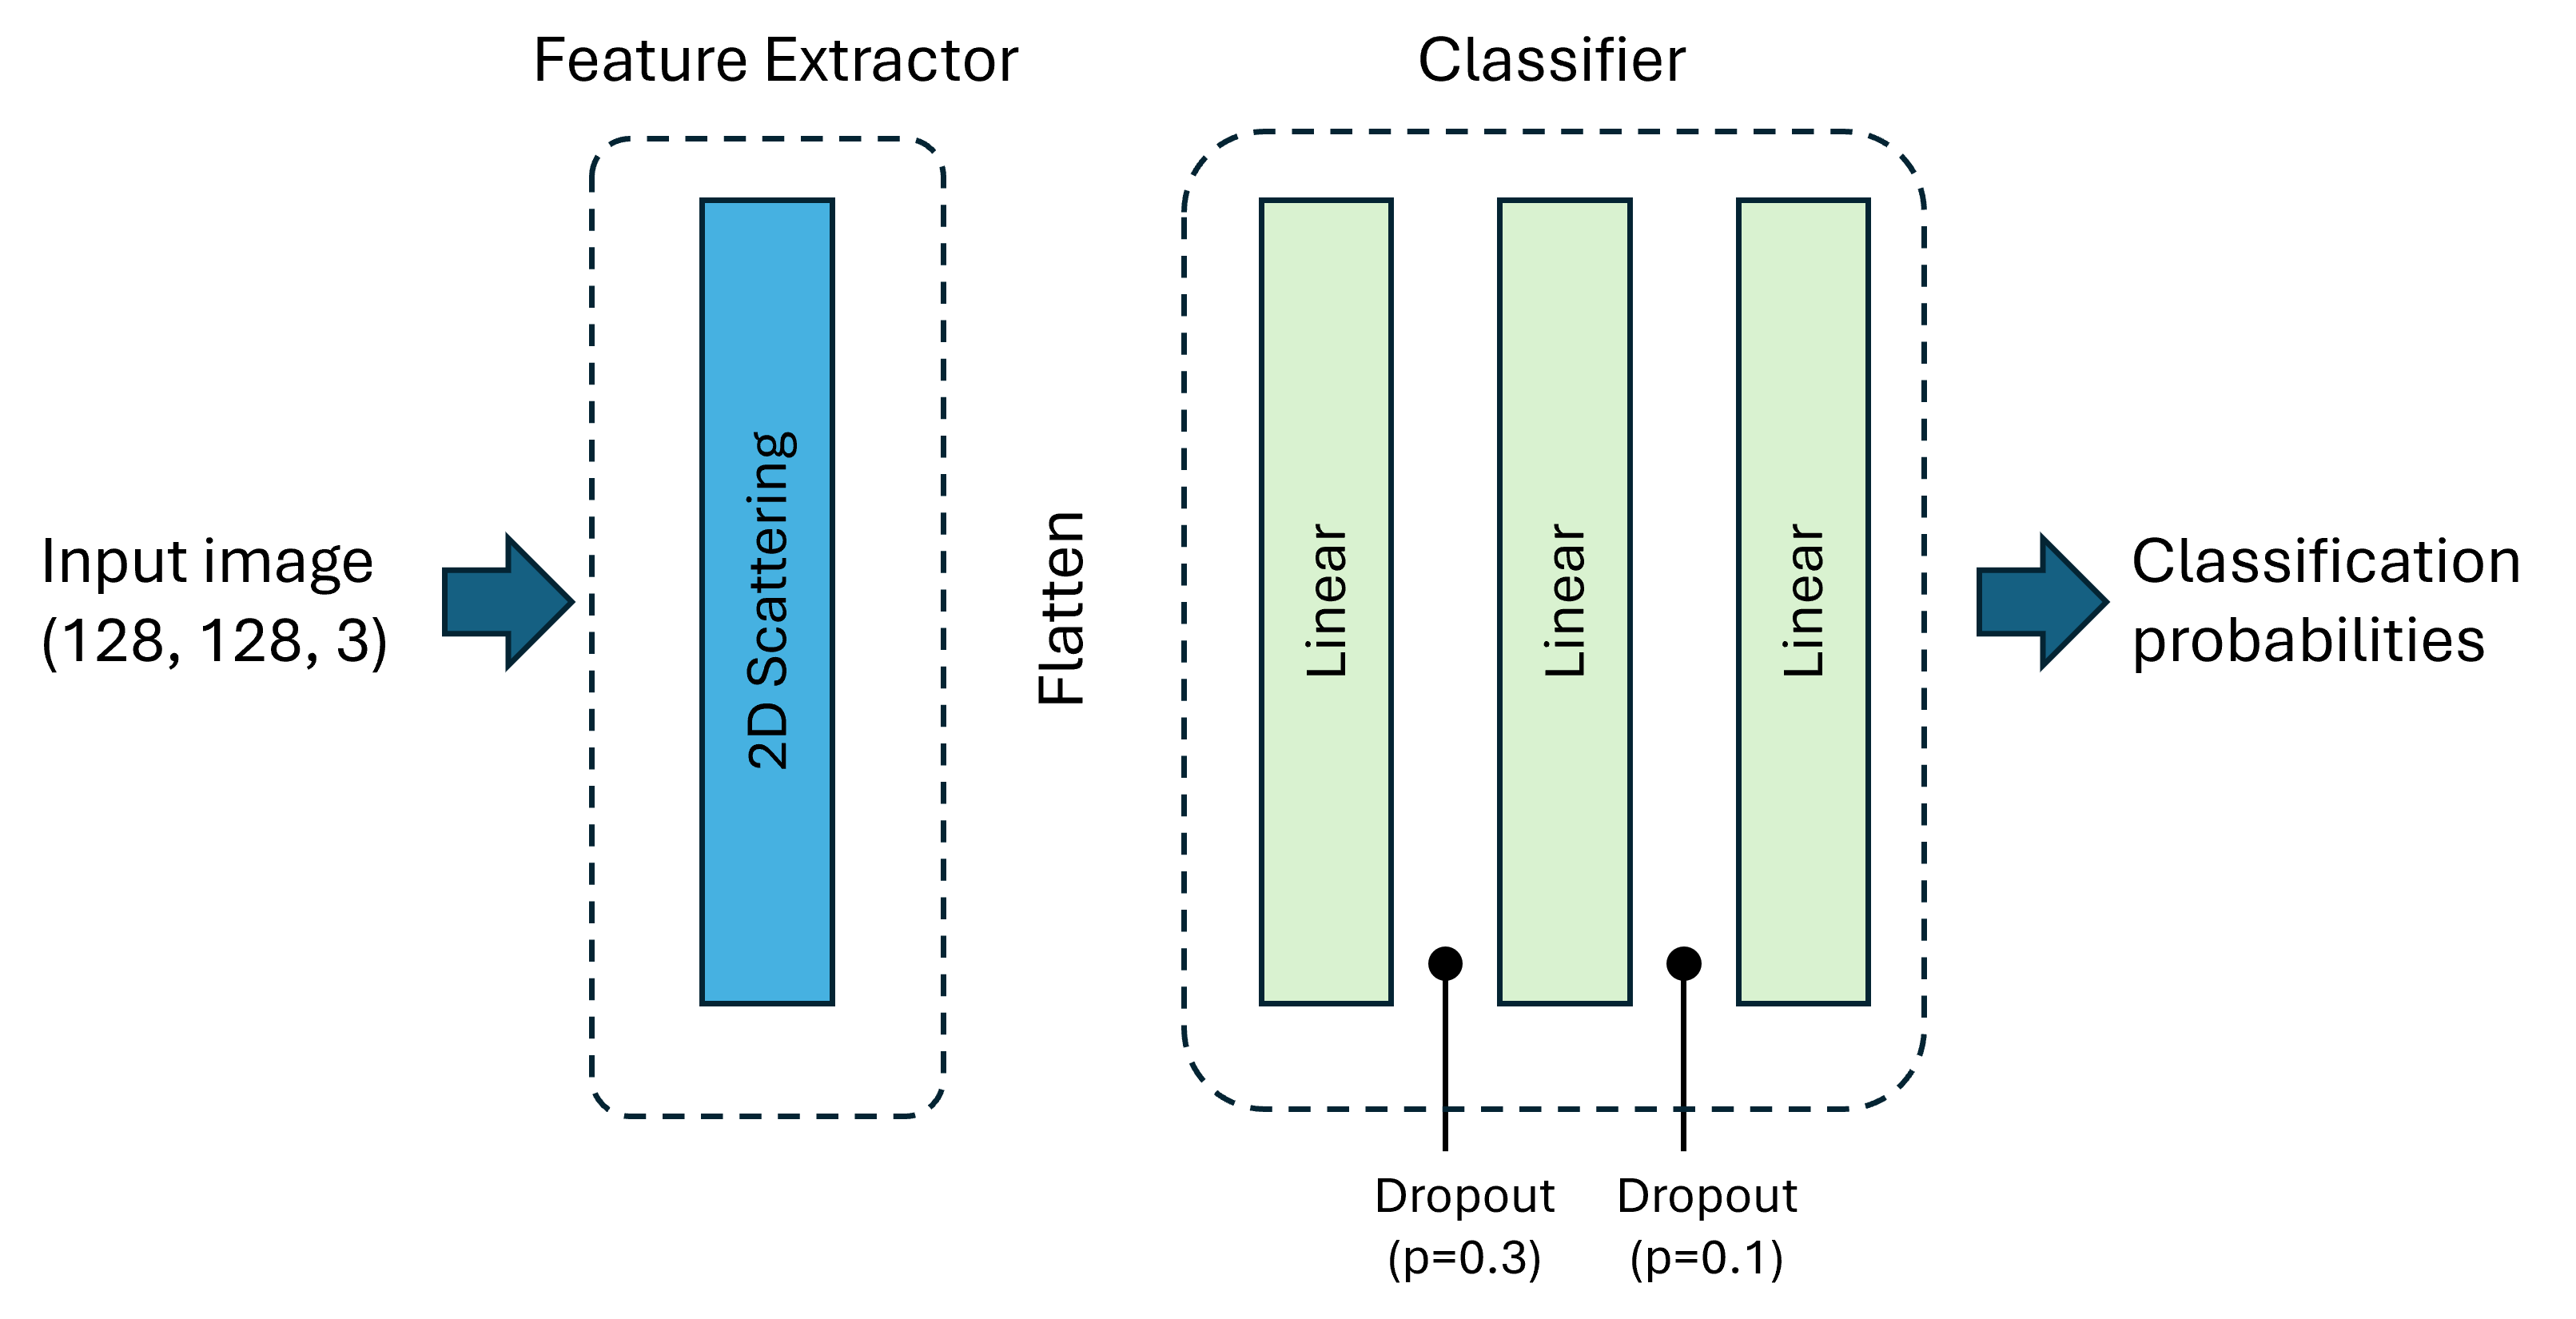
\includegraphics[width=\linewidth]{images/scatnet_architecture.png}
    \captionof{figure}{ScatNet architecture}
    \label{fig:scatnet-architecture}
\end{Figure}

% \begin{table}
%     \centering
%     \begin{tabular}{c|c|c|c|c|c}
%          \textbf{Layer} & \textbf{in feat} & \textbf{out feat} & \textbf{bias} & \textbf{\# parameters} & \textbf{activation f} \\
%          Linear & 248832 & 1024 & true & 254,804,992 & ReLU \\
%          Linear & 1024 & 1024 & true & 1,049,600 & ReLU \\
%          Linear & 1024 & 1024 & true & 2,050 & ReLU \\
%     \end{tabular}
%     \caption{Caption}
%     \label{tab1}
% \end{table}

\subsection{XAI methods}
\subsubsection{Integrated Gradients}
Integrated Gradients (IG) \cite{sundararajan2017axiomatic} is an interpretability algorithm designed to attribute predictions of a model to its input features coherently and intuitively. The fundamental idea is to integrate the gradients of the model's predictions concerning input features along a straight path from a baseline state to the actual input.

\small{$$IG_i(f,x) = (x_i - x_i') \times \int_{\alpha = 0}^1 \frac{\delta f(x' + \alpha \times (x - x'))}{\delta x_i} d\alpha$$}

\begin{itemize}
    \item $IG_i(f,x)$: the attribution of feature $i$ in input $x$ for the model $f$
    \item $x_i$: the value of feature $i$ in the input $x$
    \item $x_i'$: the value of feature $i$ in the baseline input $x'$
    \item $\frac{\delta f(x' + \alpha \times (x - x'))}{\delta x_i}$: the partial derivative of the model's prediction $f$ with respect to feature $i$ along the integration path
\end{itemize}

After choosing a baseline, the algorithm computes the gradients, integrating the model's gradients concerning each feature over a straight path from the baseline $x'$ to the actual input $x$. You have to multiply the difference between the actual and baseline feature values by the integrated gradients to obtain the attributions for each feature.

The integral represents the accumulated impact of each feature along the path. By considering this integral, Integrated Gradients offers a comprehensive understanding of the contribution of each feature to the model's prediction. This approach ensures that the attributions are both sensitive to the input values and follow a path that respects the model's decision boundaries, providing a coherent and reliable measure of feature importance.

\subsubsection{LIME - Local Interpretable Model-agnostic Explanations}
Local Interpretable Model-agnostic Explanations (LIME) \cite{ribeiro2016should} is a technique that approximates any black box machine learning model with a local, interpretable model to explain each individual prediction, to understand why the black box model made a certain prediction.

The algorithm introduces perturbations to the original data points by creating random variations in its feature space, generating a new dataset. Then it obtains predictions from the original black-box model for the new perturbed instances. 
The method then weighs those new data points as a function of their proximity to the original point. 
Ultimately, LIME fits a surrogate model (a simple, interpretable model like linear regression or decision tree) on the new dataset using those sample weights to approximate the black-box model's behavior locally. Each original data point can then be explained with the newly trained explanation model, to explain the prediction of the black-box model for a certain instance. 

More precisely, the explanation for a perturbed data point $x'$ is the model $g$ that minimizes the locality-aware loss $\mathcal{L}(f, g, \pi_x)$ measuring how unfaithful $g$ approximates the model to be explained $f$ in its vicinity $\pi_x$ while keeping the model complexity denoted low with a regularization term $\Omega(g)$.
$$\hat{f}(x') = argmin_g \mathcal{L}(f, g, \pi_x) + \Omega(g)$$
Therefore, LIME experiences a tradeoff between model fidelity and complexity. The goal of LIME algorithm is to approximate the local decision boundary of the black-box model in the vicinity of the selected instance.\\

For images the procedure to follow is different. Since more pixels are contributors for one class, it makes no sense to permutate pixels. Instead, variations of the image are created, segmenting it into superpixels. The superpixels are interconnected pixels that share some characteristics, like colors, textures or other features, and they can be altered or obscured. This step is crucial as it helps in understanding which parts of the image are influencing the model's prediction the most.
Then, you pass each perturbed image through the model and record the predictions, LIME fits an intepretable model, and the final explanation is then performed on top $n$ labels.

\section{Experiments and Results}

\subsection{Experimental Setup}
The networks were trained for 10 epochs on a machine with a Ryzen 5 5600X (6 cores, 12 threads) processor, an NVIDIA GeForce RTX 3080 Ti GPU, and with 32 Gb DDR4 of RAM. Both of the networks were trained with a learning rate of 0.001, batch size of 64, the Adam optimizer, and the cross entropy loss function.

\subsection{Metrics}
In assessing the performance of classification models, we have used accuracy and the F1 score metrics, useful for understanding the effectiveness of predictions. These metrics provide quantitative measures of correctness, precision, and recall, offering nuanced insights into the model's classification capabilities.

\subsection{CNN Experiments}
The classification results for CNN model are very good, with a good mean accuracy and f1 score in both training and validation across the 10 folds (in Table \ref{tab:cnn_training_metrics}).

\begin{table}[H]
    \centering
    \begin{tabular}{|c|c|}
        \hline
         & Mean \\
        \hline
        Train loss & 0.0489 \\
        \hline
        Val loss & 0.0567 \\
        \hline
        Train acc & 0.9840 \\
        \hline
        Val acc & 0.9813 \\
        \hline
        Train F1 & 0.9838 \\
        \hline
        Val F1 & 0.9812 \\
        \hline
    \end{tabular}
    \caption{CNN training mean metrics results averaged across the 10 folds.}
    \label{tab:cnn_training_metrics}
\end{table}

The figures show the performances of the CNN for both training and validation to see how the training was performed. In general the model goes to convergence with a spread standard deviation computed across the folds.

Testing the model, we obtain an accuracy of 94.3\% and F1 score of 94,1\% on a total of 600 test images (300 for class 0 and 300 for class 1).

\begin{Figure}
    \centering
    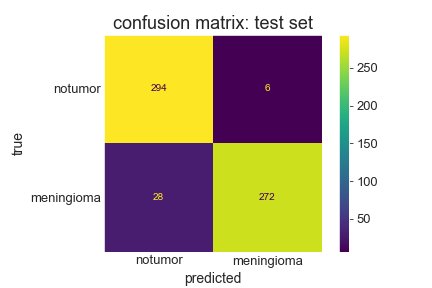
\includegraphics[width=0.75\linewidth]{images/CNN_ConfusionMatrix.png}
    \captionof{figure}{Confusion matrix for the two classes - CNN testing}
    \label{fig:cnn-confusion}
\end{Figure}

\begin{Figure}
    \centering
    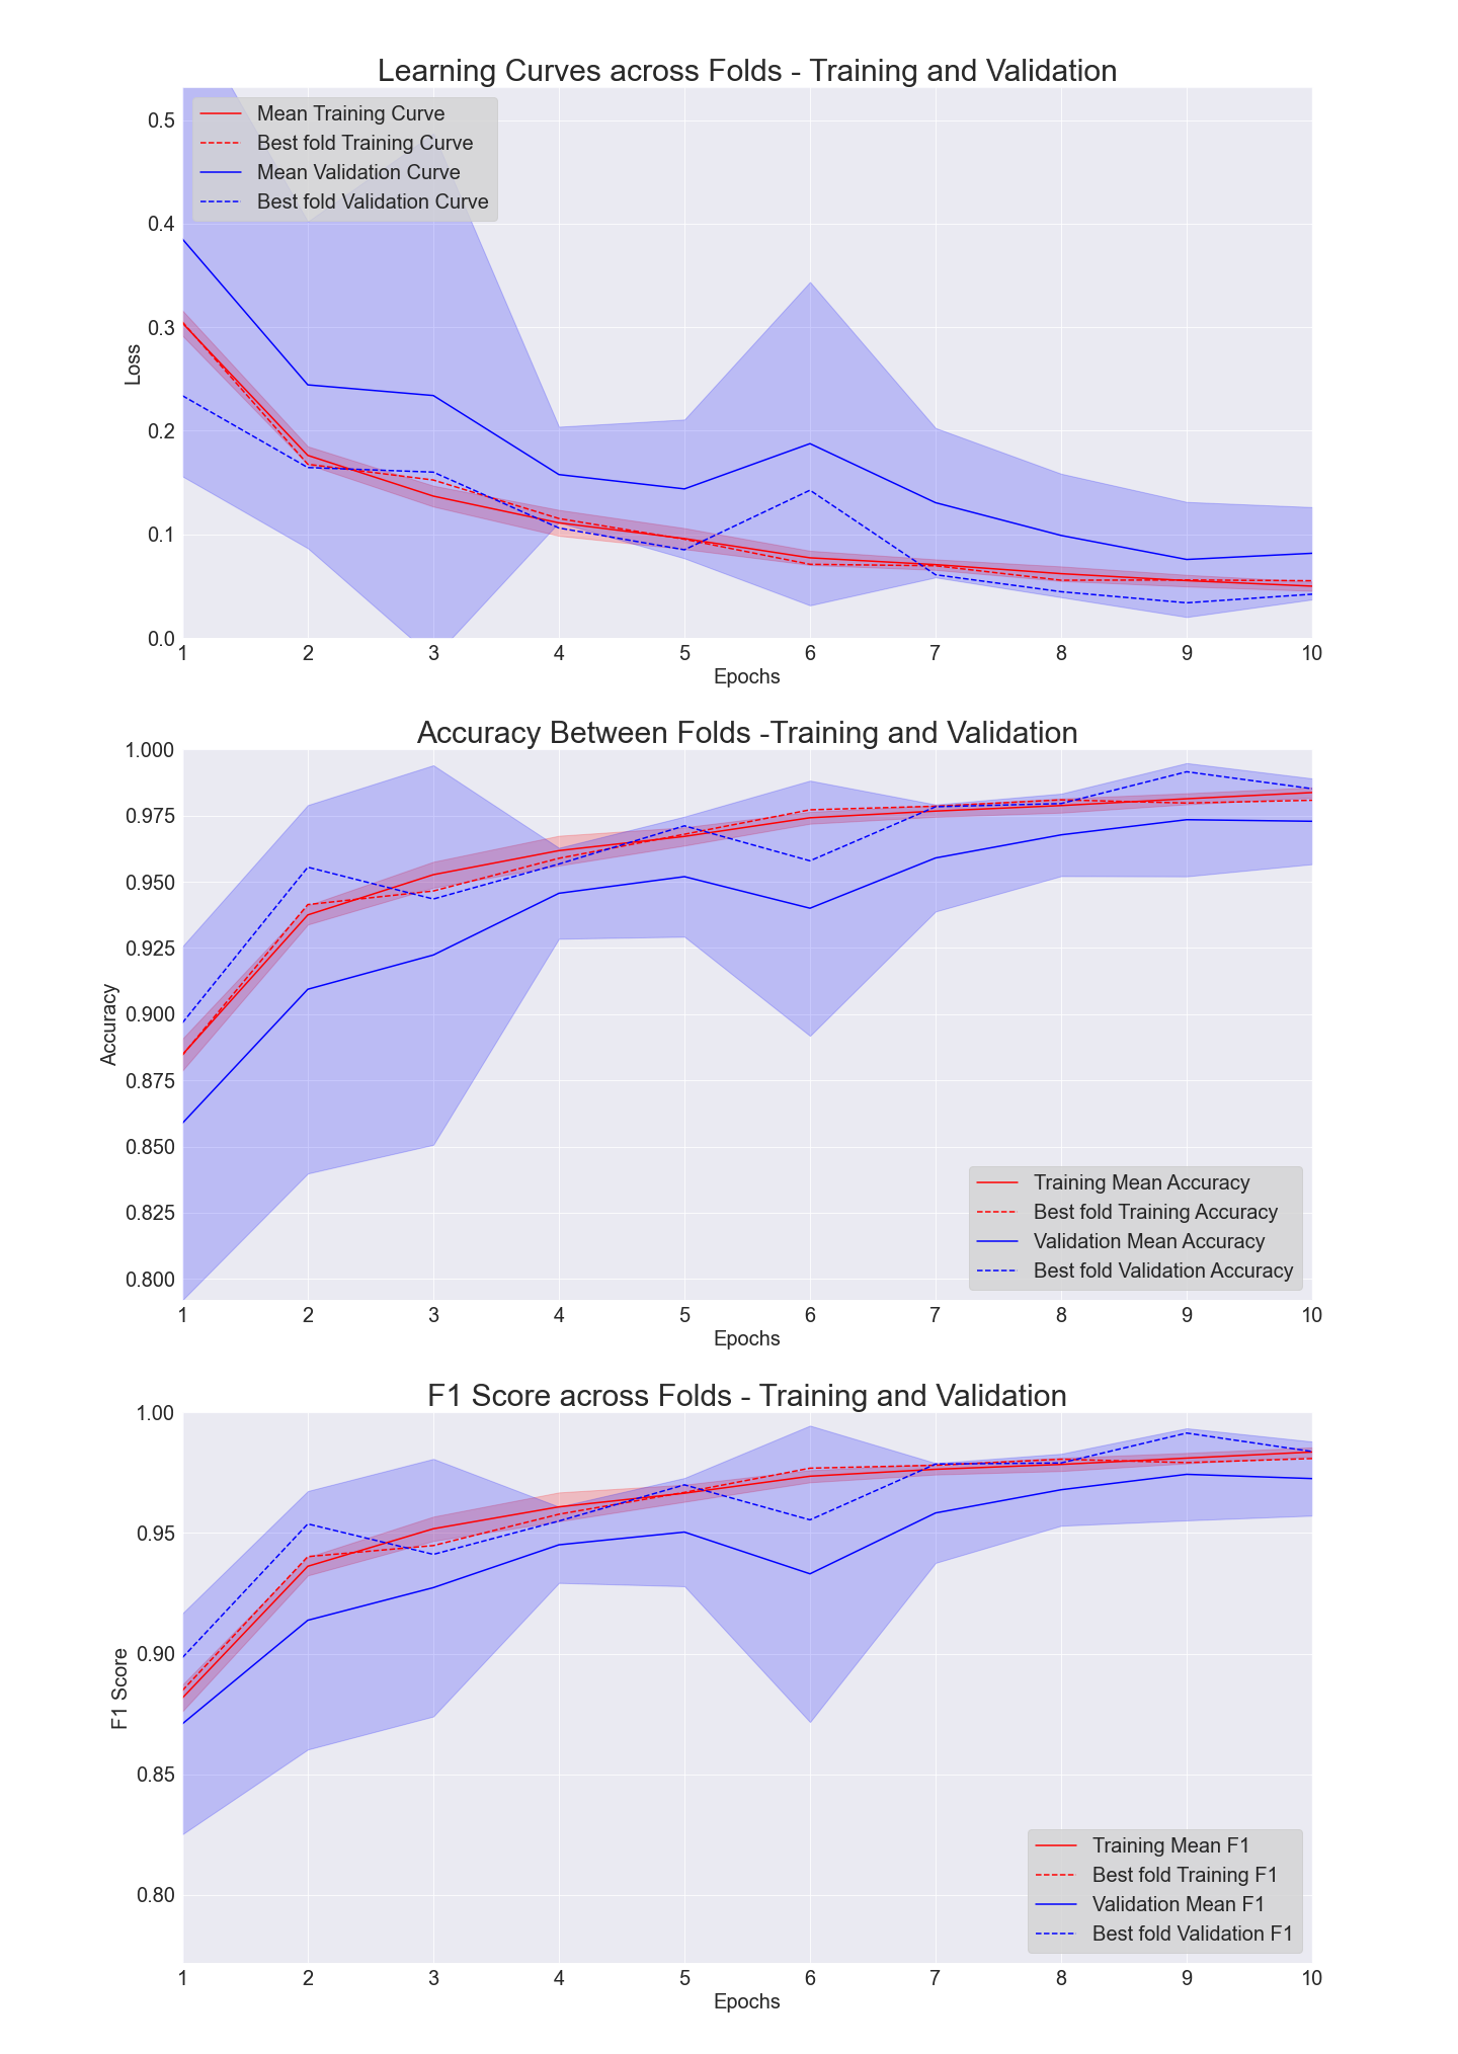
\includegraphics[width=\linewidth]{images/cnn_curves.png}
    \captionof{figure}{CNN training curves for loss, accuracy and f1 score; in red the training curves, in blue the validation curves, with both mean and best fold.}
    \label{fig:cnn-curves}
\end{Figure}


\subsection{ScatNet Experiments}
The table below shows very good results for ScatNet model, with a good mean accuracy and f1 score in both training and validation across the 10 folds (in Table \ref{tab:scat_training_metrics}), but performing worse than CNN model.

\begin{table}[H]
    \centering
    \begin{tabular}{|c|c|}
        \hline
         & Mean \\
        \hline
        Train loss & 0.1119 \\
        \hline
        Val loss & 0.1159 \\
        \hline
        Train acc & 0.9588 \\
        \hline
        Val acc & 0.9608 \\
        \hline
        Train F1 & 0.9579 \\
        \hline
        Val F1 & 0.9606 \\
        \hline
    \end{tabular}
    \caption{ScatNet training mean metrics results averaged across the 10 folds}
    \label{tab:scat_training_metrics}
\end{table}

The figures show the performances of ScatNet for both training and validation to see how the training was performed. In general, the model goes to convergence with lower standard deviations than the CNN ones in all the curves, meaning that the model is robust across the different folds.

\begin{Figure}
    \centering
    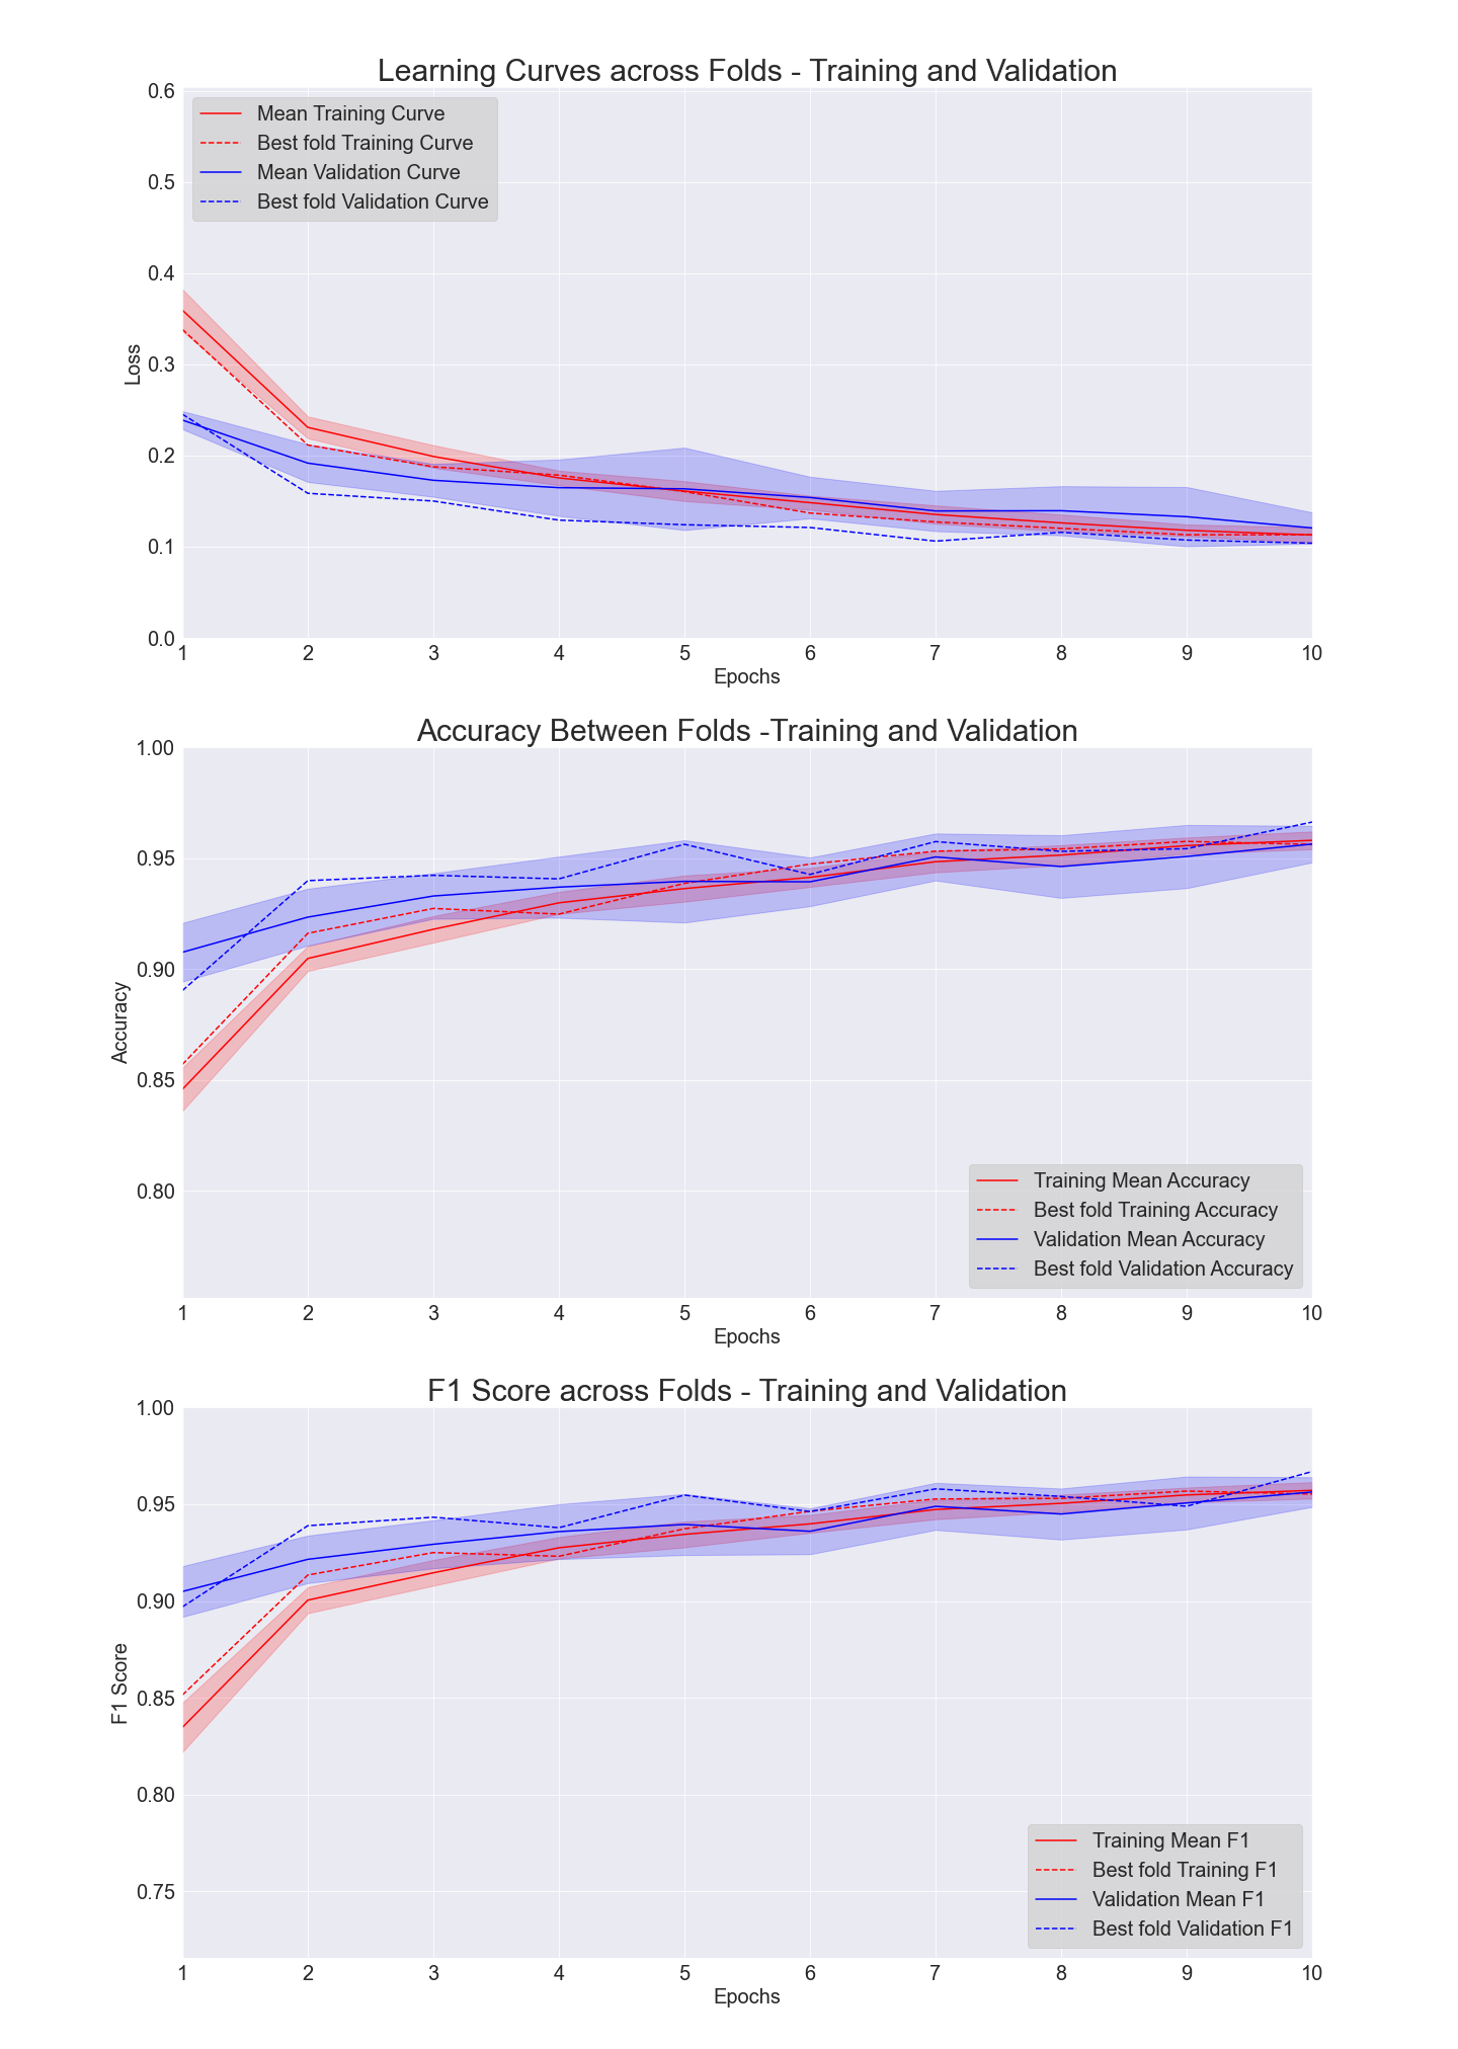
\includegraphics[width=\linewidth]{images/scatnet_curves.png}
    \captionof{figure}{ScatNet training curves for loss, accuracy and f1 score; in red the training curves, in blue the validation curves, with both mean and best fold.}
    \label{fig:scat-curves}
\end{Figure}

\begin{Figure}
    \centering
    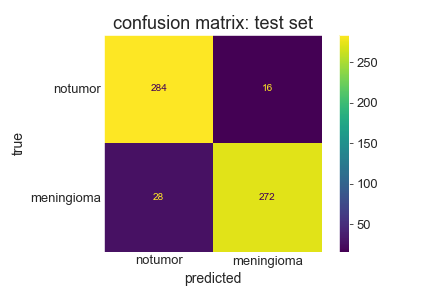
\includegraphics[width=0.75\linewidth]{images/ScatNet_ConfusionMatrix.png}
    \captionof{figure}{Confusion matrix for the two classes - ScatNet testing}
    \label{fig:scat-confusion}
\end{Figure}

Testing the model, we obtain an accuracy of 92.7\% and F1  score of 92,5\% on a total of 600 test images (300 for class 0 and 300 for class 1).
            
\subsection{Filter Extraction}
After conducting filter extraction on a chosen example image, the resulting visualizations depict the image representations at each convolutional layer (refer to Figure \ref{fig:cnn-featuremap}). Additionally, the weights, representing the kernels of the initial convolutional layer, are displayed (see Figure \ref{fig:cnn-filter}). Upon examination of these extracted filters, it is evident that certain expected features, such as distinct edge detectors or clearly defined filters, are not consistently discernible across all kernels. However, we can distinguish some of the gradients present in certain kernels. This suggests variability in the learned features within the network, prompting further investigation into the effectiveness of the training process or the architectural design of the convolutional neural network.

\begin{Figure}
    \centering
    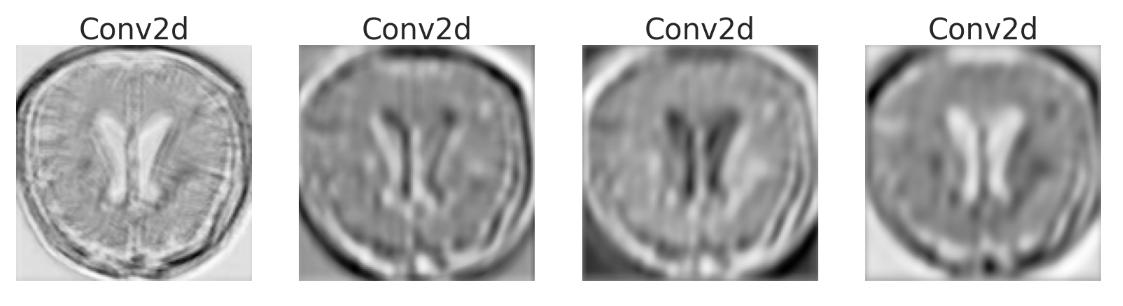
\includegraphics[width=\linewidth]{images/CNN_FeatureMaps.png}
    \captionof{figure}{Feature Maps from CNN on the example image}
    \label{fig:cnn-featuremap}
\end{Figure}

\begin{Figure}
    \centering
    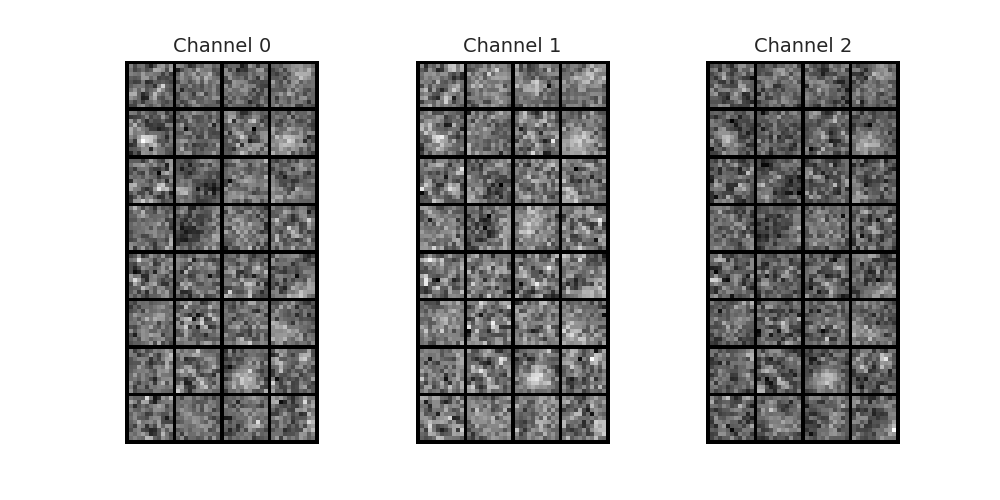
\includegraphics[width=\linewidth]{images/CNN_visTensor.png}
    \captionof{figure}{Filter extracted from the first layer of CNN}
    \label{fig:cnn-filter}
\end{Figure}

Filter extraction for ScatNet is based on the scattering transform used in the network architecture, and depends on parameters J and L set for the scattering.

\begin{Figure}
    \centering
    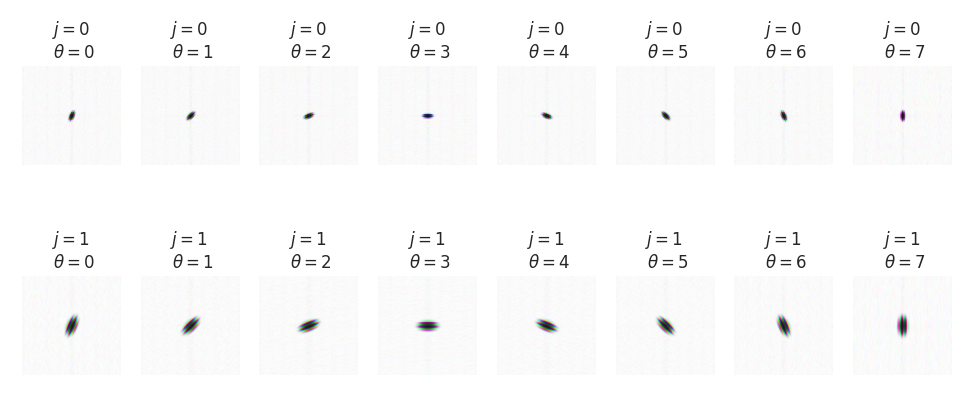
\includegraphics[width=\linewidth]{images/ScatNet_Kernels_Wavelets.png}
    \captionof{figure}{Filters extracted from ScatNet for scattering J=2 and L=8 parameters}
    \label{fig:scatnet-filter}
\end{Figure}

The filters we obtained from the two networks are not comparable for different reasons, even if ideally they have to be similar. The first reason is that the filters obtained from the ScatNet are initialized in the scattering transform based on J=2 and L=8 parameters, while CNN filters are not initialized but are based on the data. The dataset employed in our study contains images that are very similar in terms of intensity values of the pixels. Consequently, extracting significant filters from the convolutional neural network (CNN) becomes challenging. Specifically, the identification of salient gradients within filters, crucial for tasks like edge detection, becomes less pronounced due to the homogeneity in pixel intensity across images.

The second one is that we have to find always a trade-off between a good classification with significant filters and on the other side the training times and the model complexity. Considering that the model used has a simple architecture with only 4 convolutional layers and the linear classifier, and the properties of the images in the dataset, the model performs well in classification task, seeing the results in accuracy and F1 score.

\subsection{Making ScatNet better then CNN}
The two architectures were compared also changing the number of images used for training and testing. We have done an analysis based on the sistematically reduction of the number of images from 100\% of the data to 10\% of the data with a step of 10\%.

The comparison shows that in general ScatNet, starting from 50\%, performs similarly to CNN, following approximately the same trend (with a few points of difference in accuracy). Below, however, the two networks follow two different behaviours, in particular, it is seen that above 30\% CNN are much better than ScatNet, while below they are considerably worse than ScatNet, which therefore proves to be better when little data (between 10\% and 20\% of the original number of images).

This confirms what we expected: when there is few data, CNN performs worse because it is unable to generalize well and therefore is unable to learn well from a small dataset, while ScatNet, being already initialized, manages to perform better with only few data. As the number of images increases, CNN is able to learn better from the dataset while ScatNet remains at a high level considering the pre-initialized filters of the scattering transform.

\begin{Figure}
    \centering
    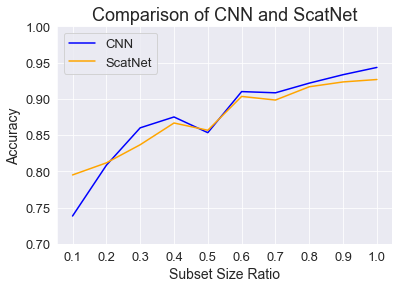
\includegraphics[width=0.8\linewidth]{images/comparison.png}
    \captionof{figure}{The figure shows the testing performances (in terms of accuracy) of both CNN and ScatNet reducing the number of data with the ratios showed.}
    \label{fig:accuracy_comparison}
\end{Figure}

\begin{Figure}
    \centering
    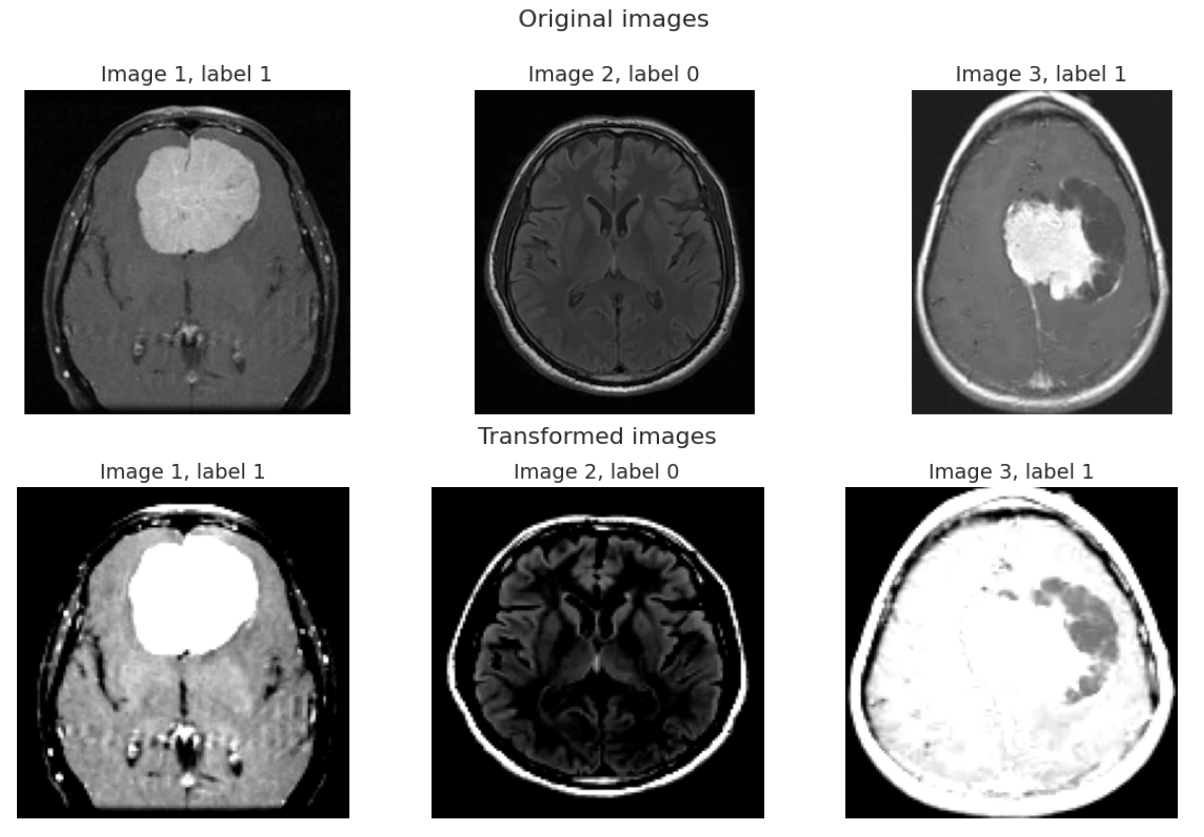
\includegraphics[width=\linewidth]{images/example_images_unified.png}
    \captionof{figure}{Images of the dataset, above the original images from the dataset, below the preprocessed ones.}
    \label{fig:example_images}
\end{Figure}

\subsection{Comparison between XAI techniques}
To assess the differences and similarities between the employed Explainable AI techniques, we report here the experiments done on three different images (Figure \ref{fig:example_images}).

\subsubsection{Integrated Gradients}
\paragraph{Baseline choice} 
To get the most out of the Integrated Gradients algorithm the first step is to choose an adequate baseline. The optimal baseline was defined as the input signal for which the prediction of the network held maximum uncertainty. We tried three different baselines: Zeros baseline, Uniform baseline, and Mean Baseline, for a neutrality check (the results are shown in the table 2 for each model). The best baseline from the three we've tried is the zeros baseline because it's the nearest one to the neutrality 50-50.

\begin{Figure}
    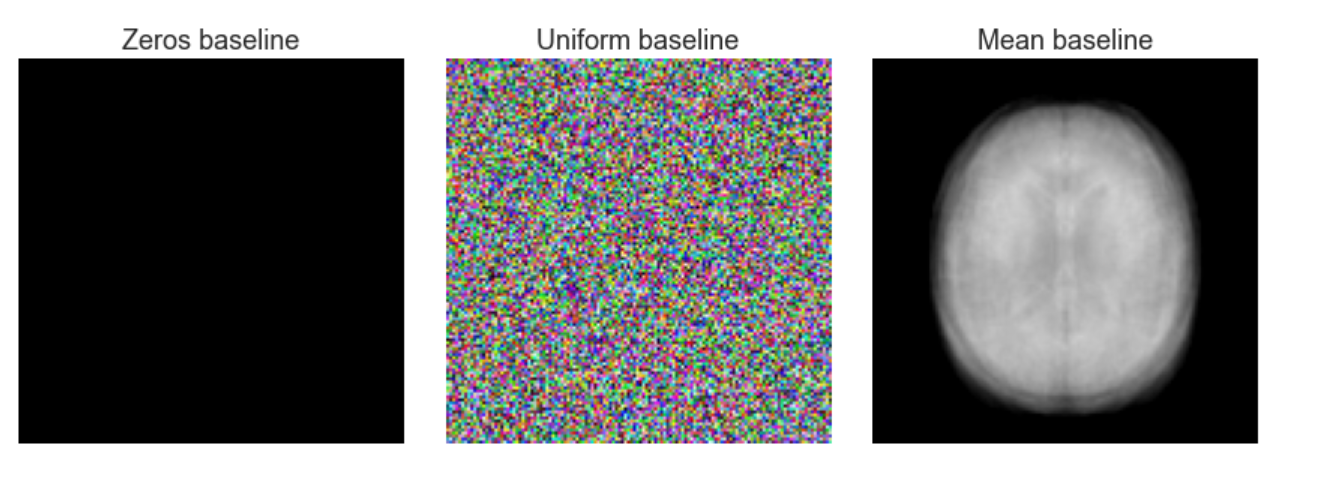
\includegraphics[width=\linewidth]{images/baseline.png}
    \captionof{figure}{Zero baseline, Uniform noise baseline and Average input data baseline.}
    \label{fig:baseline}
\end{Figure}

\begin{table}[H]
    \centering
    \begin{tabular}{|c|c|c|}
        \multicolumn{3}{c}{CNN Model} \\
        \hline
        Baseline & Class 0 & Class 1 \\
        \hline
        Zeros & 0.2290 & 0.7710 \\ 
        Uniform & 0.9853 & 0.0147 \\
        Mean & 0.9988 & 0.0012 \\
        \hline
    \end{tabular}
    \label{tab:neutrality1}
    \vspace{0.2cm}
    \begin{tabular}{|c|c|c|}
        \multicolumn{3}{c}{ScatNet Model} \\
        \hline
        Baseline & Class 0 & Class 1 \\
        \hline
        Zeros & 0.4637 & 0.5363 \\ 
        Uniform & 0.9850 & 0.0150 \\
        Mean & 0.0172 & 0.9828 \\
        \hline
    \end{tabular}
    \label{tab:neutrality2}
    \caption{Tables shown the result of neutrality check performed on 3 different baselines: zeros baseline, uniform noise baseline, and mean baseline (computed as mean of all data). The table shows the probabilities of predicting one of the two class by testing each baseline for both networks.}
\end{table}

One of the instances of Integrated Gradients was implemented from scratch, following the original paper \cite{sundararajan2017axiomatic}, while the other one is an implementation of the library \texttt{Captum} \cite{captum}. Here we show the differences between the baseline, the original images and the results from the two algorithms for the two networks. 

\begin{Figure}
    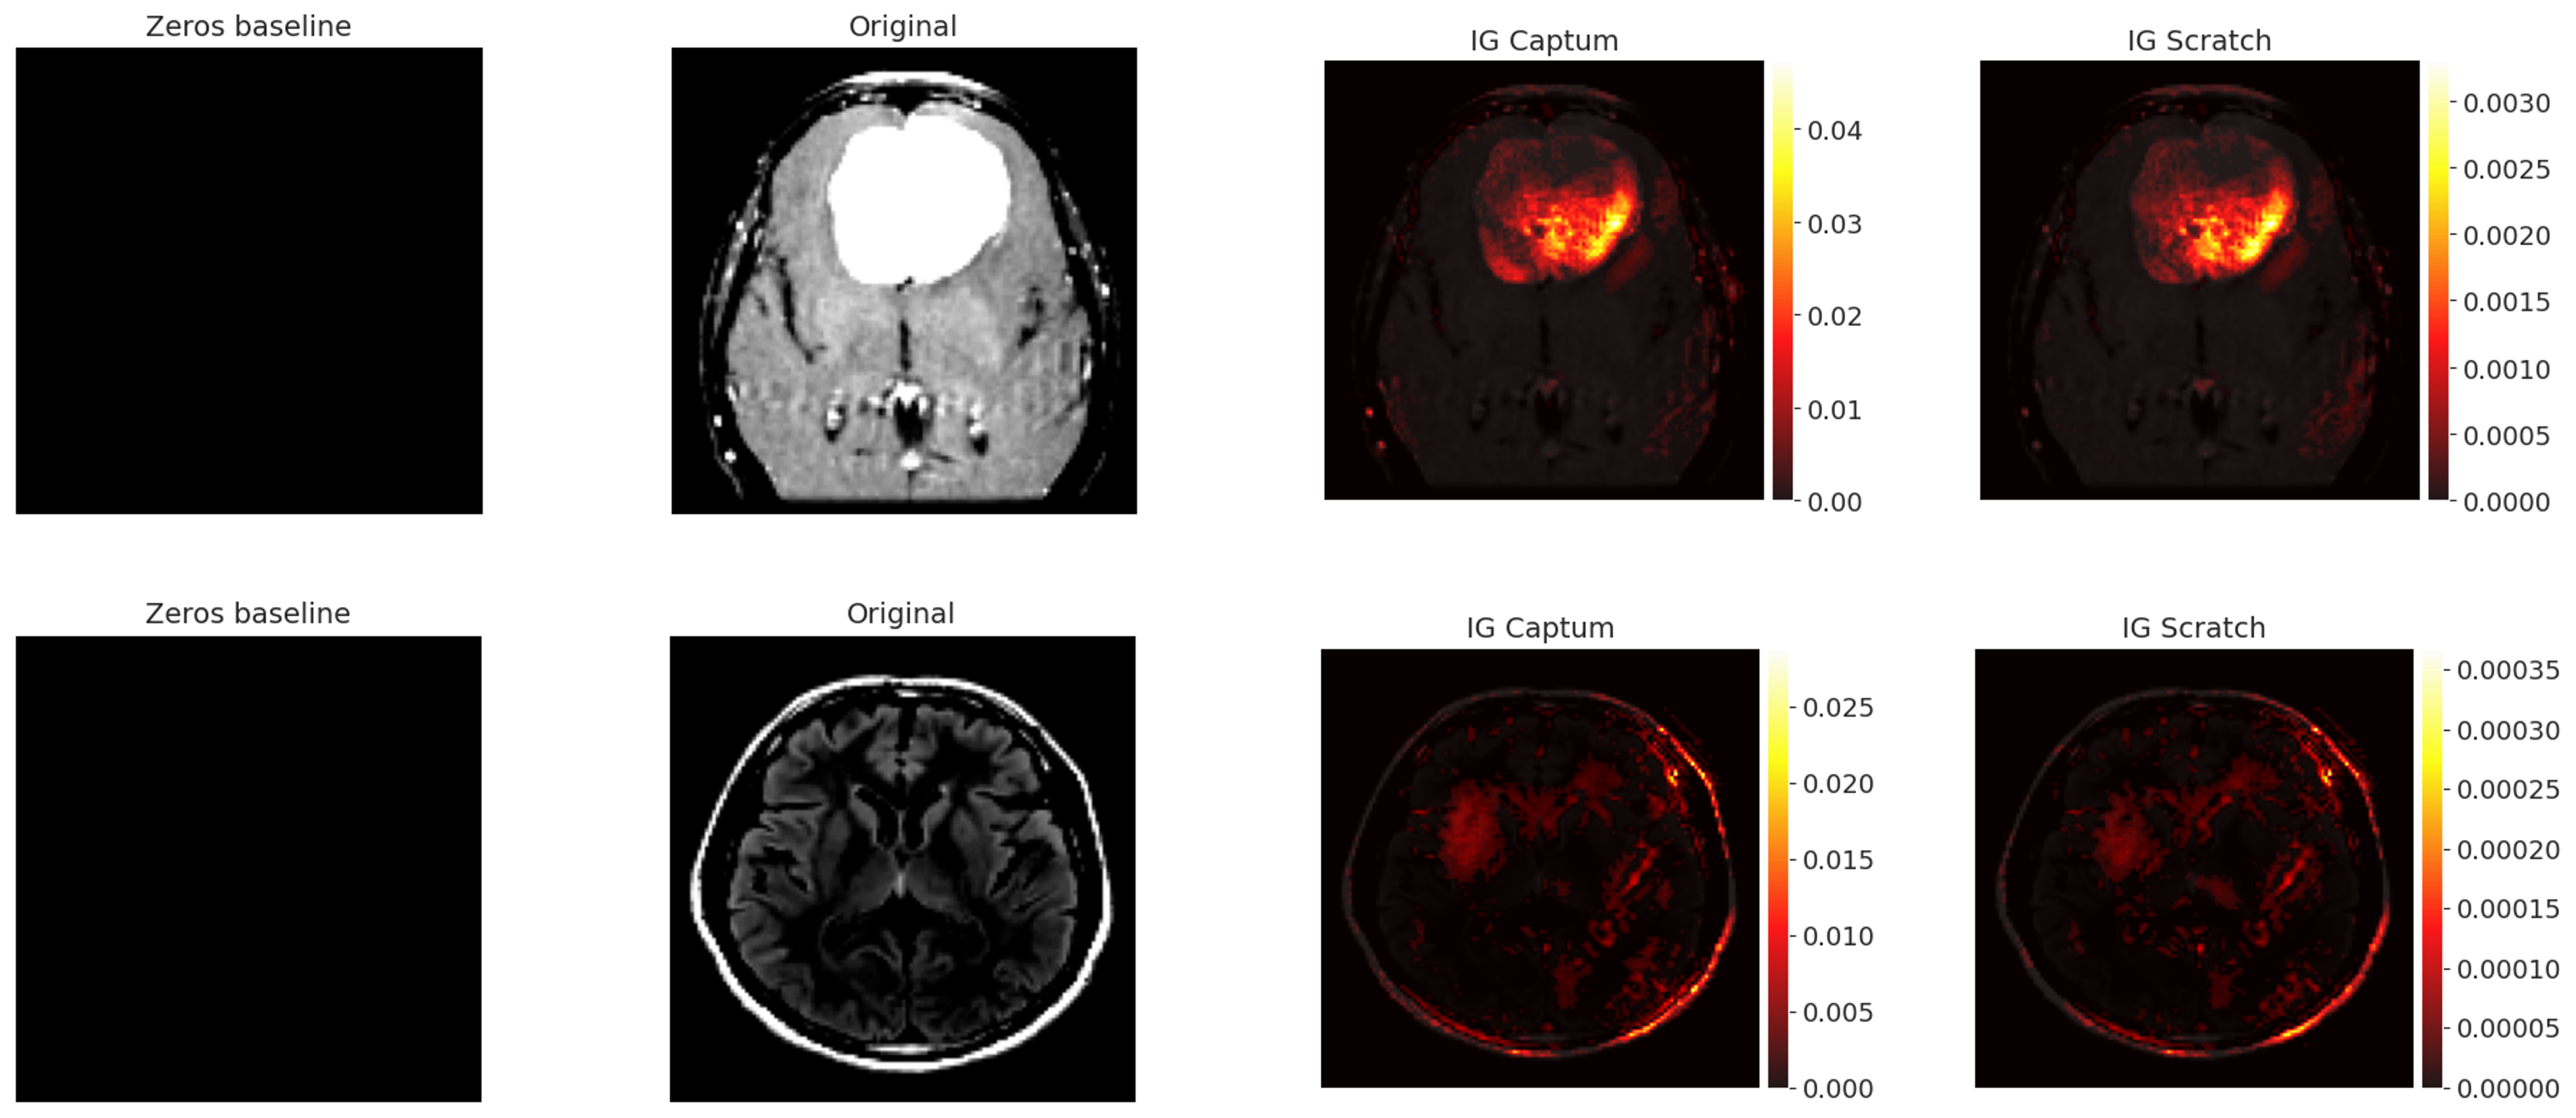
\includegraphics[width=\linewidth]{images/IG_CNN.png}
    \captionof{figure}{Integrated Gradient from Scratch and using Captum, with zero baseline for CNN model; above the image with tumor (class 1) and below the image without tumor (class 0).}
    \label{fig:integrated-gradients-cnn}
\end{Figure}

\begin{Figure}
    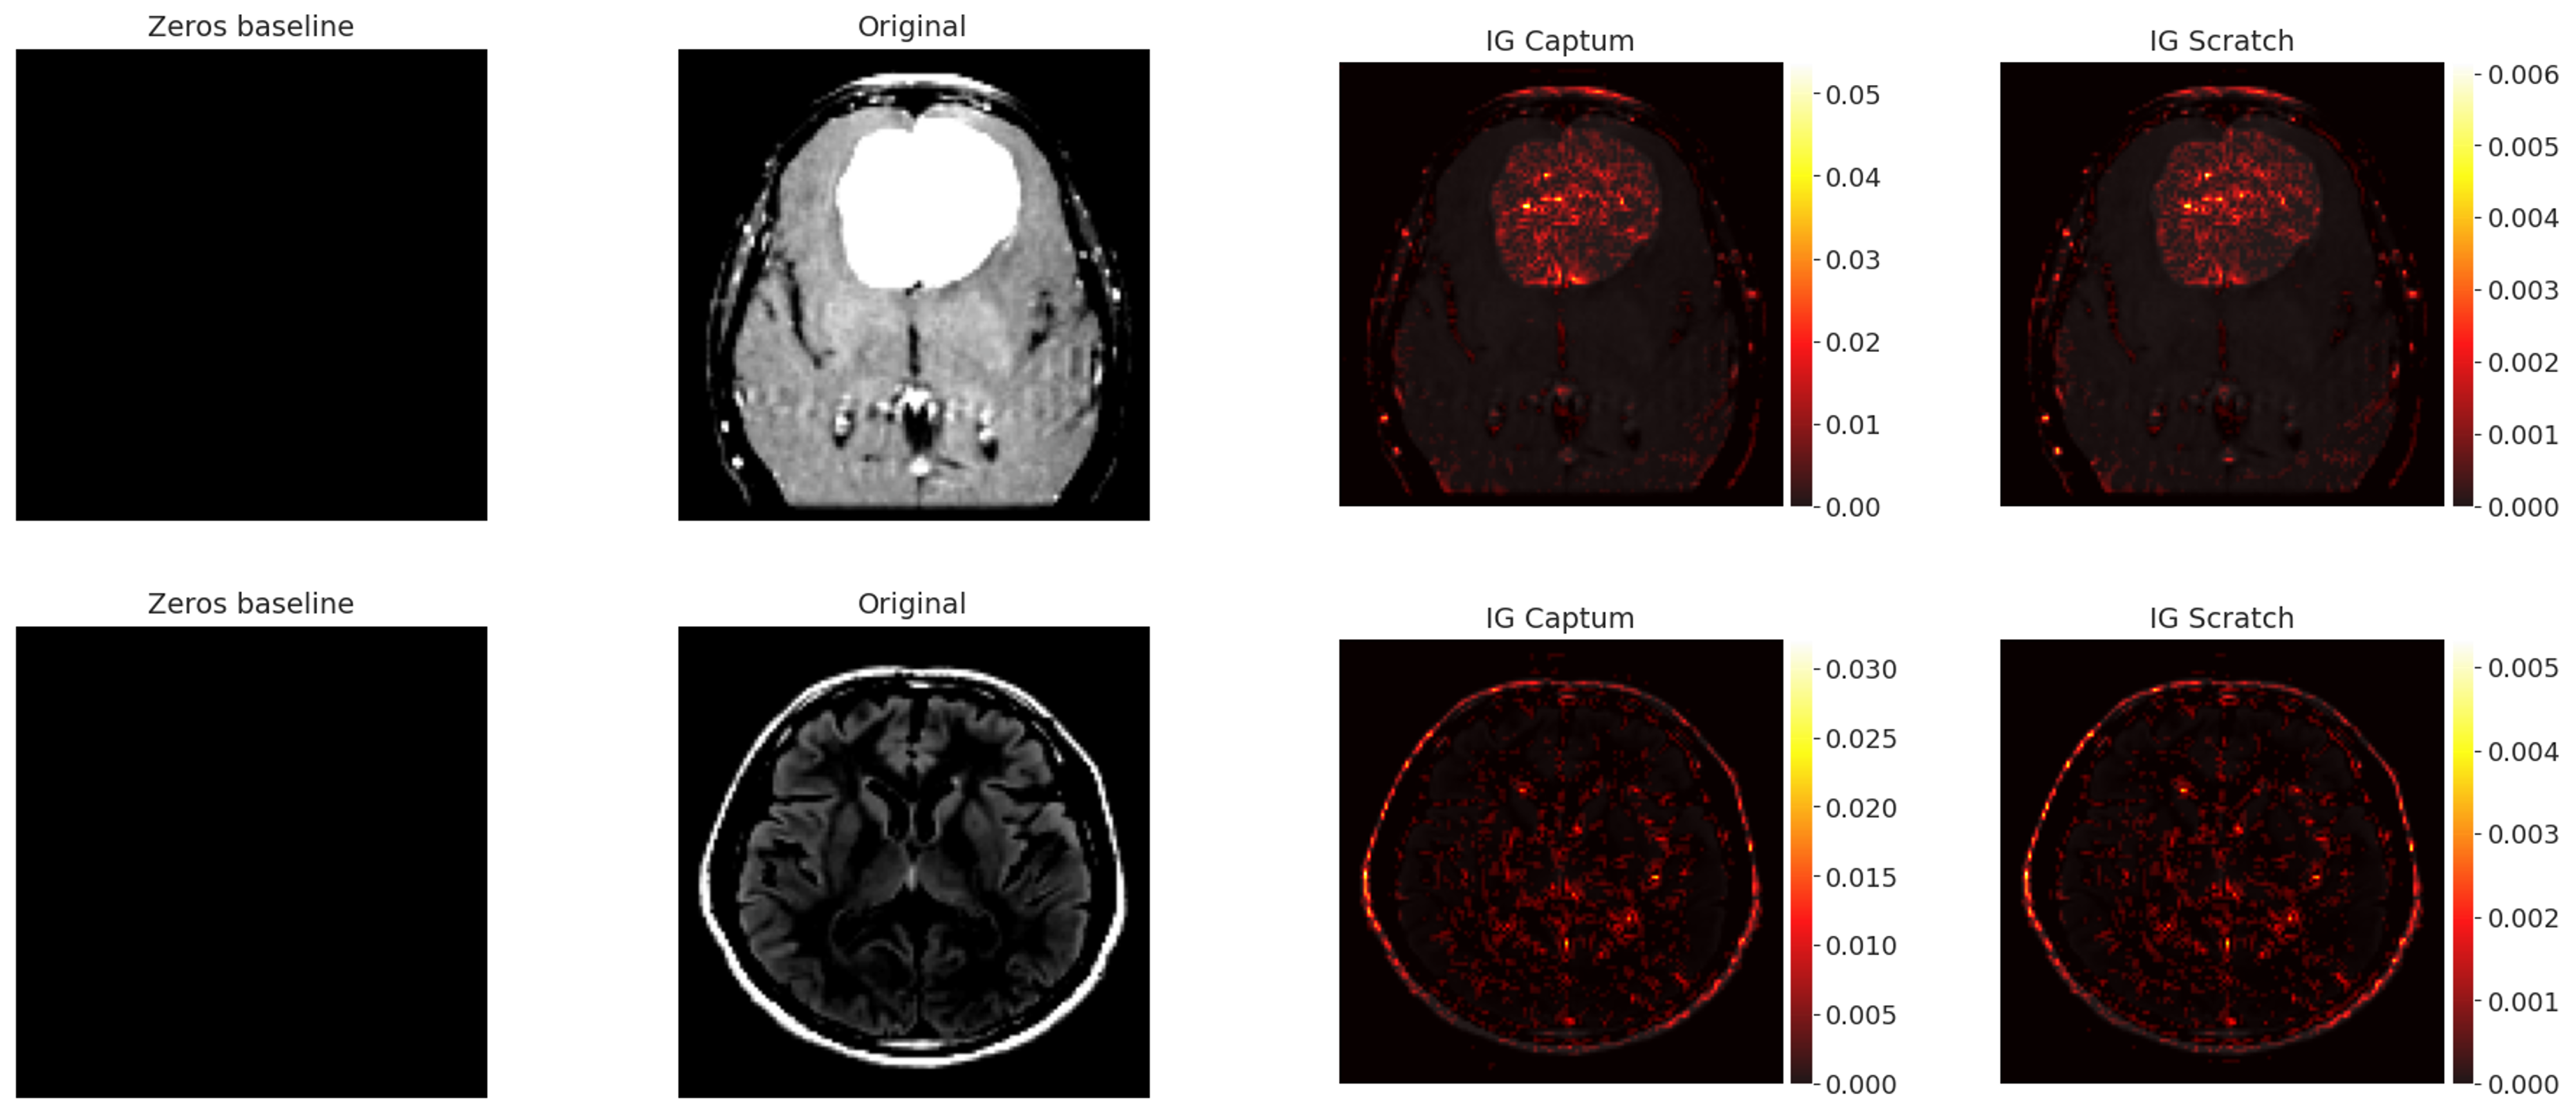
\includegraphics[width=\linewidth]{images/IG_SCATNET.png}
    \captionof{figure}{Integrated Gradient from Scratch and using Captum, with zero baseline for ScatNet model; above the image with tumor (class 1) and below the image without tumor (class 0).}
    \label{fig:integrated-gradients-scatnet}
\end{Figure}

As you can see from Figure \ref{fig:integrated-gradients-cnn} for CNN and Figure \ref{fig:integrated-gradients-scatnet} for ScatNet, for both models, in both implementations of the Integrated Gradients (from the \texttt{Captum} library and from scratch) it is clearly seen that in the first example the attributions are concentrated on the tumor area, which is therefore detected very well, while in the example without tumor the attributions are more distributed in the image, in some cases focusing more on the scalp.

\subsubsection{LIME}
The same three images used for Integrated Gradients were also explained by LIME, in this case the implementation is only one, from the python library \texttt{lime} \cite{limepackage}.

\begin{Figure}
    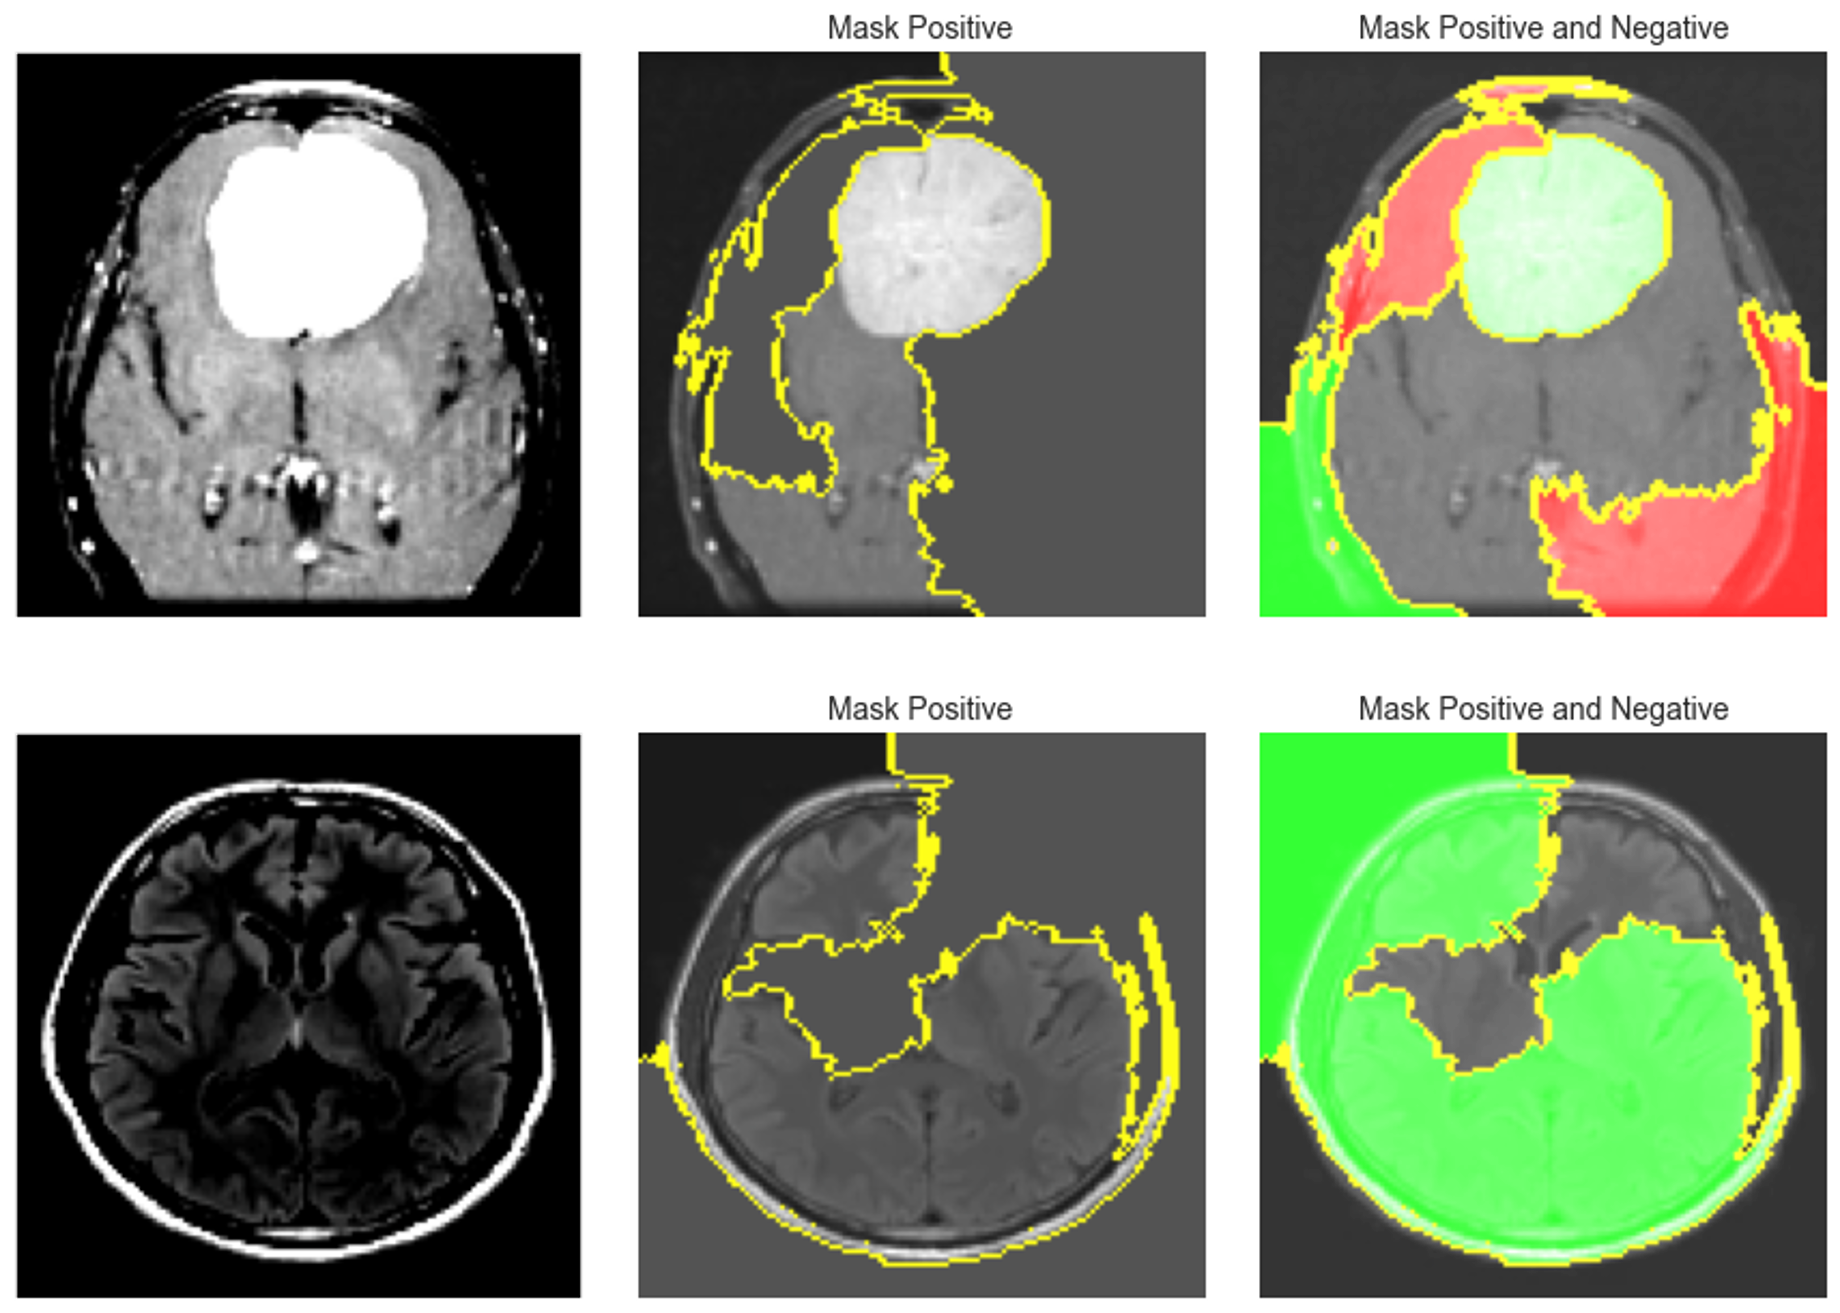
\includegraphics[width=\linewidth]{images/cnn_lime.png}
    \captionof{figure}{LIME performed for CNN model with only positive superpixel and with positive and negative superpixel. Above an example with tumor; below an example without tumor.}
    \label{fig:LIME-cnn}
\end{Figure}

\begin{Figure}
    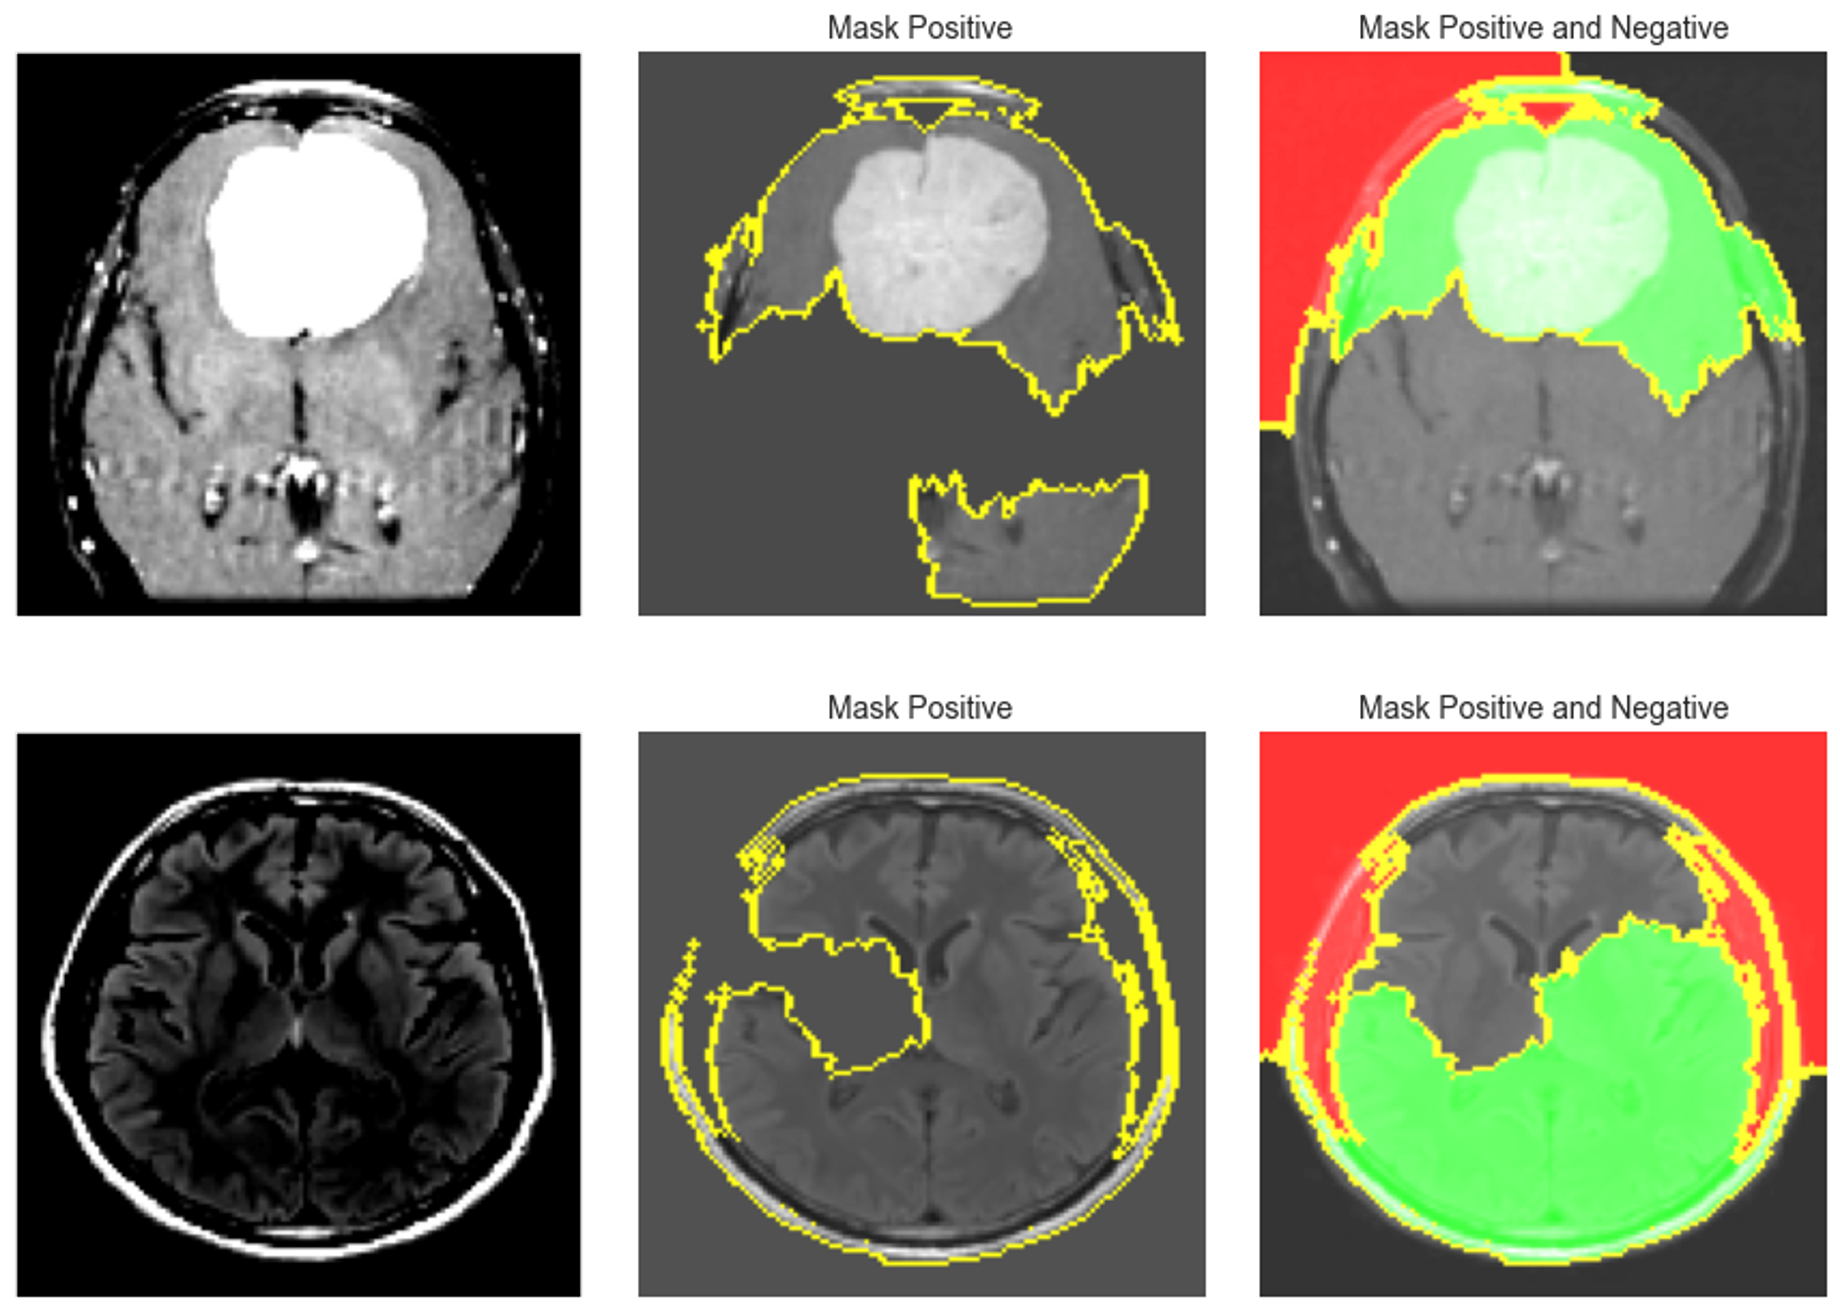
\includegraphics[width=\linewidth]{images/scatnet_lime.png}
    \captionof{figure}{LIME performed for ScatNet model with only positive superpixel and with positive and negative superpixel. Above is an example of an image of the tumor class; below is an example without tumor.}
    \label{fig:LIME-scat}
\end{Figure}

From Figure \ref{fig:LIME-cnn} for the CNN model and Figure \ref{fig:LIME-scat} for the ScatNet model, we can see that the algorithm manages to detect the tumor correctly, assigning positive values to the tumor area for the correct class, both for the CNN model and for the ScatNet model.


\subsection{Statistical analysis}
Statistical analysis was done on the results of the attribution maps obtained from Integrated Gradients (from scratch and \texttt{Captum} library) and LIME algorithms for the three test images. In particular, we've computed the histograms of the attribution maps, the correlation between the attribution maps of the different algorithms, and the mutual information metric.

\paragraph{Histogram Analysis}
For visualization purposes, we've normalized the values of the attributions for all the methods. Analyzing the resulting images (Figures \ref{fig:cnn-histograms}, \ref{fig:scat-histograms}) we understand that the two versions of Integrated Gradients have the same distributions. On the other hand, LIME shows the characteristic peaks of the mask (green, red, and none that originally were represented by values 1, -1, and 0)

%%% Histograms
\begin{Figure}
    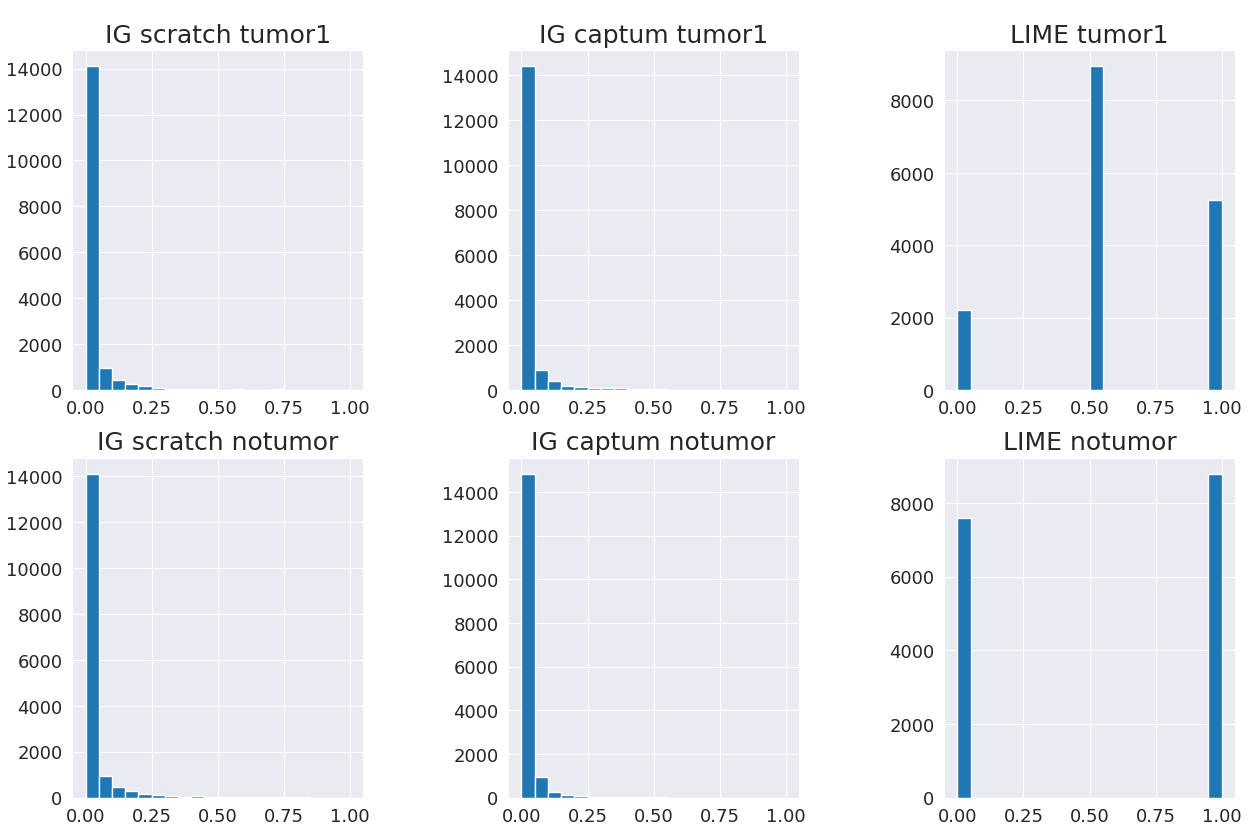
\includegraphics[width=\linewidth]{images/cnn_histograms.png}
    \captionof{figure}{Histogram of attribution maps obtained from images with and without tumor for    CNN model.}
    \label{fig:cnn-histograms}
\end{Figure}

\begin{Figure}
    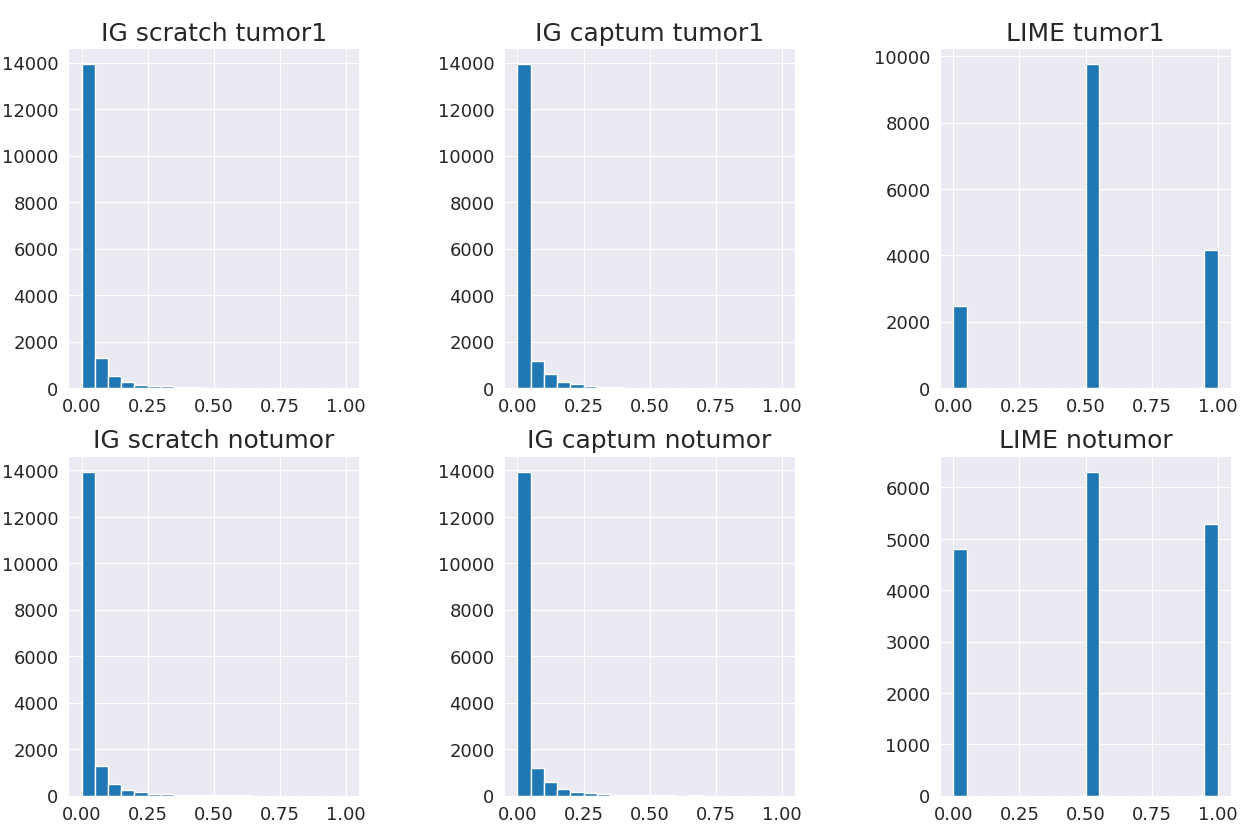
\includegraphics[width=\linewidth]{images/scatnet_histograms.png}
    \captionof{figure}{Histogram of attribution maps obtained from images with and without tumor for    ScatNet model.}
    \label{fig:scat-histograms}
\end{Figure}


%%% Correlation
\begin{Figure}
    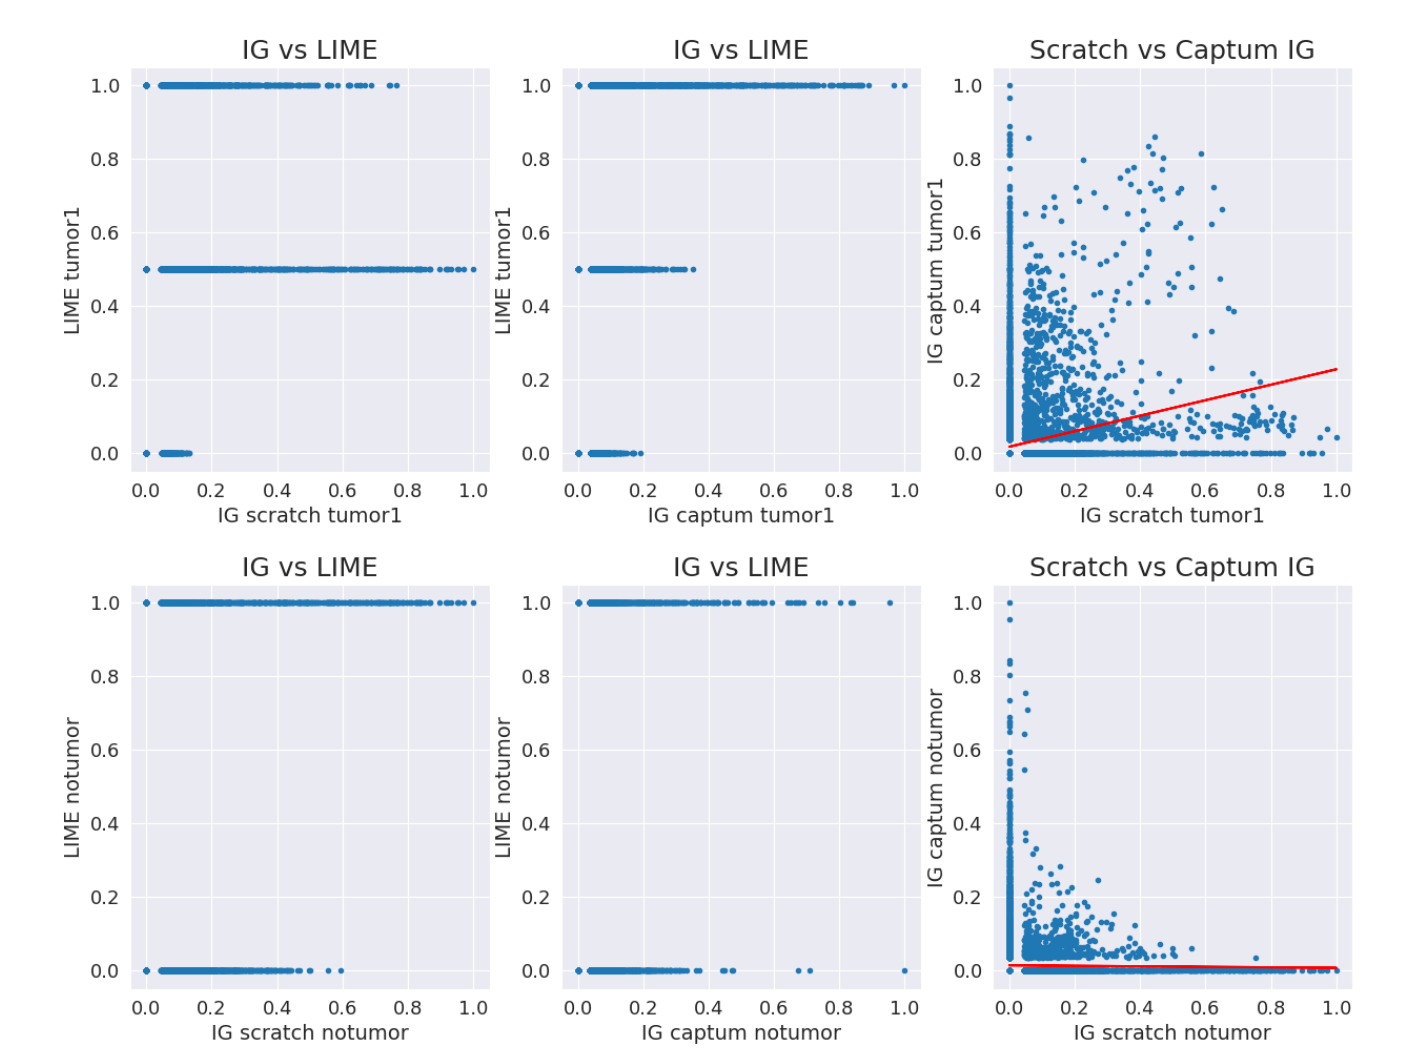
\includegraphics[width=\linewidth]{images/cnn_correlation.png}
    \captionof{figure}{Correlation between attribution maps obtained from images with and without tumor for CNN model.}
    \label{fig:cnn-correlation}
\end{Figure}

\begin{Figure}
    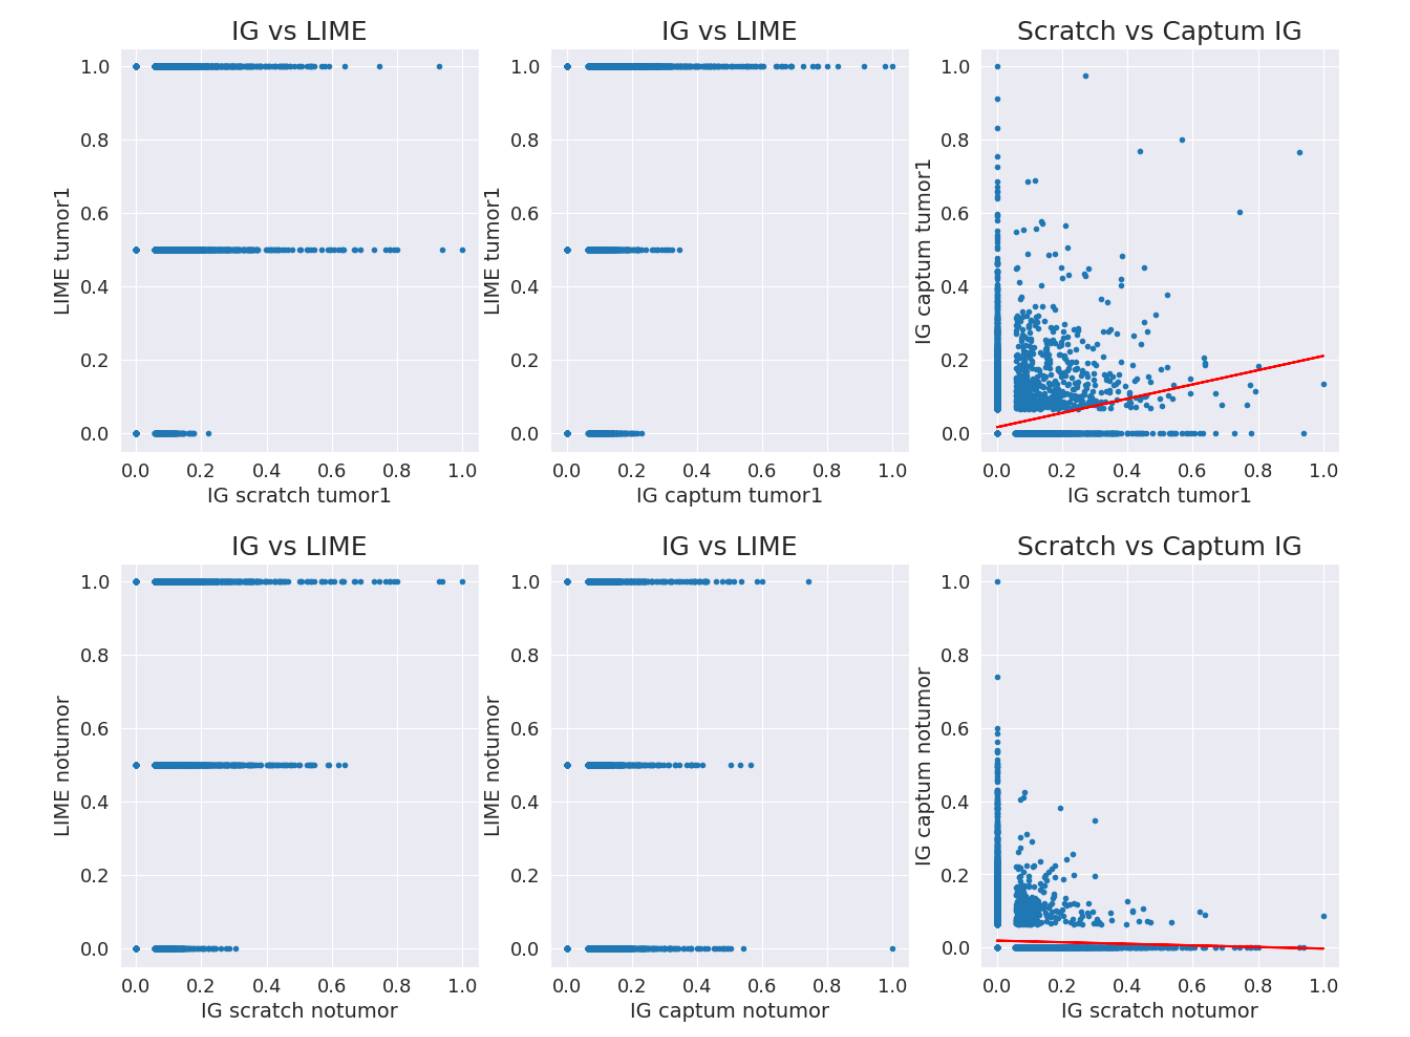
\includegraphics[width=\linewidth]{images/scatnet_correlation.png}
    \captionof{figure}{Correlation between attribution maps obtained from images with and without tumor for ScatNet model.}
    \label{fig:scat-correlation}
\end{Figure}


\paragraph{Correlation Analysis}
Each point on the scatter plots represents an instance (e.g., a single pixel) in our images (Figures \ref{fig:cnn-correlation}, \ref{fig:scat-correlation}). The position of a point on the plot indicates how the attributions from the two methods we're analyzing correlate for that instance. We can state that in all of the scatter plots regarding the confrontation of one of the two implementations of Integrated Gradients with LIME, we can identify straight lines, suggesting that the methods' attributions are closely related. However, there is a consistent difference between the plots that confront the two implementations of Integrated Gradients: while we can roughly identify two lines, it's evident that they differ. 

In these two plots, we can also identify a wide spread between the points, which indicates that the methods’ attributions vary significantly for different pixels. We can conclude that, while the attributions seem to identify stable and relevant features, especially around extreme values (black and white), they widely disagree on various other pixels. On the contrary, they both seem to agree with LIME.


\section{Discussion and Conclusions}
The analysis aimed to compare two architectures, CNN and ScatNet, from the point of view of performance and explainability applied to a dataset of brain images with and without tumor. The results show that in general the CNN model performs better than the ScatNet model in terms of accuracy considering the entirety of the chosen dataset, while ScatNet performs better than CNN when the dataset is reduced to 10\% of the original. 

Trying to explain and interpret the models with XAI algorithms - Integrated Gradients and LIME -, it seems that the first method makes more clear the presence of the tumor, when present. On the other hand, LIME seems to be highlighting a wider pixel area than the one implicated, concerning also underlying pixels that are not relevant to the tumor identification.

In conclusion, the two models used perform well in terms of classification performance and it can be seen quite clearly how they have learned to correctly distinguish the relevant parts of the images of the dataset for the correct prediction.

\newpage
\printbibliography

% \begin{thebibliography}{9}

% \bibitem{shap}
% Lundberg, Scott M., and Su-In Lee. \emph{A unified approach to interpreting model predictions}, Advances in neural information processing systems 30 (2017).

% \bibitem{ig}
% Sundararajan, Mukund, Ankur Taly, and Qiqi Yan. \emph{Axiomatic attribution for deep networks}, International conference on machine learning. PMLR, 2017.

% \bibitem{lime}
% Ribeiro Marco Tulio, Sameer Singh, and Carlos Guestrin. \emph{"Why should I trust you?" Explaining the predictions of any classifier}, Proceedings of the 22nd ACM SIGKDD international conference on knowledge discovery and data mining. 2016.

% \end{thebibliography}

\end{multicols*}

\end{document}
